\documentclass[a4paper,12pt]{article}
\usepackage[utf8]{inputenc}
\usepackage[MeX]{polski}
\usepackage{graphicx}
\usepackage{sidecap}
\usepackage{wrapfig}
\usepackage{subfig}
\usepackage{amsfonts}
\usepackage{amssymb}
\usepackage{float}
\usepackage{latexsym}
\newtheorem{twr}{Definicja}
\newtheorem{tw}{Twierdzenie}
\newpage
\thispagestyle{empty}
\begin{center}
\textbf{\large Uniwersytet Wrocławski\\
Wydział Matematyki i Informatyki\\
Instytut Matematyczny}\\
\textit{\large specjalność: Matematyka stosowana}\\
\vspace{4cm}
\textbf{\textit{\large Magdalena Wawrzyniak}\\
\vspace{0.5cm}
{\Large Automaty komórkowe w równaniach różniczkowych cząstkowych.}}\\
\end{center}
\vspace{3cm}
{\large \hspace*{6.5cm}Praca licencjacka\\
\hspace*{6.5cm}napisana pod kierunkiem\\
\hspace*{6.5cm}prof. dr hab. Grzegorz Karch }\\
\vfill
\begin{center}
{\large Wrocław 2020}\\
\end{center}

\begin{document}
\newpage
\textbf{Streszczenie}\\\\
Celem pracy licencjackiej ,,Automaty komórkowe w równaniach różniczkowych cząstkowych.” jest pokazanie, że równania różniczkowe cząstkowe są ogromnym źródłem automatów komórkowych. Praca rozpoczyna się od zebrania i uporządkowania podstawowych informacji na temat automatów komórkowych. Pierwsza połowa pracy skupia się na dokładnym zdefiniowaniu automatów komórkowych, klasyfikacji oraz przypomina najpopularniejsze automaty komórkowe. Kolejnymi aspektami omówionymi w pracy są automaty komórkowe pochodzące od równań różniczkowych, takich jak równanie dyfuzji lub reakcji-dyfuzji. Istotną częścią pracy są również kody stworzone w języku R, który umożliwiły przetestowanie automatów komórkowych w praktyce i stworzenie licznych symulacji, które możemy oglądać w pracy. Całość kończy bibliografia. \\\\

\textbf{Abstract}\\\\
Aim of Bachelor thesis "Cellular Automata in partial differential equations" is to show that partial differential equations are a big source of cellular automata. Thesis begins with gathering and sorting basic information about cellular automata. First half of this work focuses on precisely defining cellular automata, classification and reminds us of the most popular cellular automata. Next thing spoken of in the thesis are cellular automata derived from differential equations, like diffusion equation or reaction-diffusion. Important part of this thesis are code examples written in R programming language, which were used to put exemplary cellular automata to a test and to create numerous simulations, which we can observe in my work. Thesis ends with bibliography.

\newpage
\tableofcontents
\newpage
\section{Wprowadzenie}
Na początek, zanim poznamy formalną definicję automatów komórkowych, dobrze będzie nabyć pewną intuicję, która pomoże w ogólnym zrozumieniu, czym automaty komórkowe właściwie są, gdzie możemy się ich doszukiwać. \\
Automaty komórkowe są to modele, w których wszystkie zmienne przyjmują dyskretne wartości, które są ściśle związane z lokalizacją komórki i jej najbliższym sąsiedztwem. Dla lepszego zrozumienia tematu możemy zobrazować to, na przykładzie pożarów lasu lub rozprzestrzeniania się infekcji. Jeżeli w lesie zostanie podłożony ogień, to zacznie się on rozprzestrzeniać na pobliskie drzewa, ale jeżeli ogień będzie za mały lub będzie za daleko obserwowanego przez nas obszaru, to w tym miejscu las się nie podpali. Tak samo jeżeli ogień będzie zbyt duży, to bardzo szybko się wypali. W przypadku infekcji, jeżeli w klasie będzie jedna chora osoba, to najprawdopodobniej jej znajomy z ławki również zachoruje i tak samo inne osoby, z którymi miała ta osoba bezpośredni kontakt. \\
Za tymi przykładami kryją się pewne "lokalne" zasady, które dyktują dynamikę rozprzestrzeniania się bodźca (ogień, infekcja). Odpowiedzmy, więc sobie na pytanie, czym jest przestrzeń, w której on się rozchodzi. W tych modelach przestrzeń reprezentowana jest przez pojedyncze punkty, nazywane komórkami, które możemy interpretować na dwa sposoby. Komórkę możemy utożsamiać z miejscem, na którym żyje osobnik/zjawisko lub jako osobnika samego w sobie. \\
Przytoczone przeze mnie przykłady są jednymi z wielu sytuacji, w których możemy odszukać i zaprojektować automaty, co chętnie wykorzystuje się w biologii. Pierwszy z powodów tego stanu rzeczy został sformułowany już na początku mojej pracy, a mianowicie to, że modele są dyskretne. Jest to istotne z tego względu, że ogromna ilość struktur badanych przez biologów jest dyskretna, co przekłada się na ich opis. Po drugie, algorytm jest stosunkowo prosty do zaprogramowania, a w zamian dostarcza nam sporo ciekawych informacji i umożliwia nam obserwacje w skali globalnej skutków działania w obrębie mikrostruktur. Trzecim równie ważnym powodem, przez który automaty są chętnie wykorzystywane jest to, że bardzo dobrze odzwierciedlają przebieg biologicznych zjawisk w czasie.\\
Automaty komórkowe zawdzięczają swój początek węgierskiemu uczonemu John'emu von Neumann'owi, który około 1952 roku opracował, przy użyciu papieru milimetrowego i ołówka, pierwszy automat, który przedstawiał zjawisko samoreplikacji~\cite[s. 155]{hill}. Matematyk zastanawiał się nad tym, jak z jednego złożonego systemu może powstać inny system o takiej samej złożoności. W tamtych latach było to rewolucyjne odkrycie, zwłaszcza że nie znano jeszcze strukturalnej budowy DNA, nie wspominając o samym przebiegu replikacji DNA. Jeszcze bardziej zadziwiający powinien być fakt, że model, który von Neumann zaprojektował, posiadał aż 29 stanów, które mogła przyjąć komórka, a początkowe konfiguracje były rozpisywane aż dla 200 000 komórek~\cite[s. 155, 156]{hill}. W dzisiejszych czasach przeprowadzanie takich obliczeń jest niewyobrażalne bez użycia komputera.\\
Brak odpowiednich narzędzi w dużej mierze ograniczył rozwój w tym zakresie, czego skutkiem była niewielka ilość publikacji. Świat nauki musiał poczekać, aż pojawi się maszyna o odpowiedniej mocy obliczeniowej i na tyle przystępna w obsłudze, aby temat mógł pójść naprzód. Automaty komórkowe zaczęły przeżywać swój renesans, wraz z powstaniem "Gry w życie" John'a Conway'a i spopularyzowaniem jej na łamach miesięcznika popularnonaukowego Scientific American, przez dziennikarza Martin'a Gardner'a~\cite{g}. Gra wzbudziła ciekawość wśród ludzi tym, że losowe układy początkowe, wraz z przebiegiem gry ewoluowały, w niespotykany do tej pory sposób. Wiele osób poza rozrywką dostrzegła możliwości, jakie dają automaty.  

\section{Matematyczna definicja zagadnienia}
Ten rozdział został napisany na podstawie książki \cite[s.156,157]{hill}
Mamy już ogólne pojęcie, czym są automaty komórkowe. Aby omówić je bardziej szczegółowo, wprowadźmy ich definicję.
\begin{twr}
Automat komórkowy jest to uporządkowana czwórka $A=(G,E,U,f)$, gdzie:
\begin{itemize}
    \item $G$ - siatka komórek,
    \item $E$ - zbiór stanów elementarnych,
    \item $U$ - zbiór zdefiniowanych sąsiadów,
    \item $f$ - lokalne zasady.
\end{itemize}
\end{twr}
Sama definicja może nie jest zbyt jasna, więc pokrótce omówimy sobie każdą składową $A$:\\
\begin{enumerate}
    \item W klasycznym automacie komórkowym $G=\mathbb{Z}^d$, gdzie $d$ oznacza wymiar siatki.
    \item Punkty kratowe siatki będziemy przedstawiać jako komórki.
    \item $E$ to zbiór stanów, jakie może przyjąć każda komórka, np. $E=\{0,1\}$ lub $E=\{biały,czarny\}$, gdzie $0$ lub "biały" może reprezentować "martwą" komórkę, a $1$ lub "czarny" "żywą".
\end{enumerate}


\begin{twr}
Niech $A=(G,E,U,f)$ będzie automatem komórkowym. Wtedy przez $U(x)$ będzie oznaczać sąsiedztwo komórki $x$, gdzie $x\notin U(x)$. 
\end{twr} W literaturze możemy trafić na dwie różne interpretacje, w jednej $x$ będzie należał do sąsiedztwa, a  w innych nie musi się tak zdarzyć. W drugim wymiarze, najpowszechniejszymi sąsiedztwami są sąsiedztwa von Neumanna oraz  Moore'a, które pokazano na rysunku 1.\\
\begin{figure}
\centering
\subfloat[sąsiedztwo von Neumanna]{\label{odnosnik}
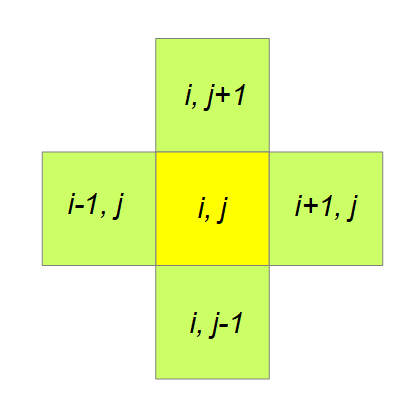
\includegraphics[width=0.33\textwidth]{vonneumann.png}}
\quad
\subfloat[sąsiedztwo Moore'a]{\label{odnosnik}
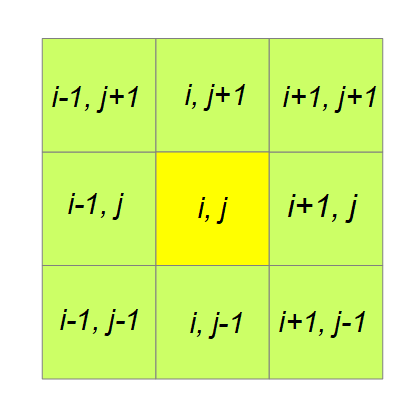
\includegraphics[width=0.3\textwidth]{moore.png}}
\caption{}
\end{figure}
\begin{twr}
Przez $\tau(x,t)$ będziemy oznaczali stan komórki $x$ w czasie $t$. Nowy stan komórki $x$ jest zależny tylko i wyłącznie od stanów sąsiednich komórek:
$$\tau(x,t+1)=f(\tau(\cdot,t)|_{U(x)}),$$
gdzie $\tau(\cdot,0)$ to stan początkowy wszystkich komórek. Wyrażenie $\tau(\cdot,t)$ informuje o stanach wszystkich komórek w kroku $t$.
\end{twr}
Funkcja $f$ odpowiada za przejście komórki $x$, ze stanu $\tau(x,t)$ do $\tau(x,t+1)$, gdzie w argumencie podajemy sąsiedztwo $x$, a na wyjściu otrzymamy nowy stan w kolejnym kroku.\\

\section{Klasyfikacja automatów komórkowych}
Informacje zamieszczone w tej części zostały napisane na podstawie rozdziału 6.1.1. z książki \cite{hill}.

\subsection{Podział automatów komórkowych}
W połowie lat osiemdziesiątych brytyjski naukowiec Stephan Wolfram zaproponował sposób w jaki możemy klasyfikować automaty komórkowe. Wyróżnił on cztery klasy, a o przynależności do danej z nich świadczy sposób w jaki rozwija się w czasie obserwowany przez nas automat.
\begin{description}
\item[Klasa I:] Z każdej konfiguracji początkowej otrzymujemy stałe punkty, czyli wzór staje się stały w czasie.
\item[Klasa II:] Proste stacjonarne lub okresowe struktury ewoluują, a małe zmiany stanu początkowego wpływają tylko na skończoną liczbę komórek.
\item[Klasa III:] Wyłaniają się chaotyczne i pseudolosowe wzory. Liczba komórek, na które wpływają zmiany w stanie początkowym wzrasta liniowo wraz z upływem czasu.
\item[Klasa IV:] Rozmieszczenie wzorów długofalowo wpływa na następne konfiguracje, a efekt zmian dla stanu początkowego jest trudny do przewidzenia. 
\end{description}
Każdy z automatów możemy przydzielić do jednej z powyższych klas, spróbujmy znaleźć po jednym reprezentancie z każdej klasy. Przykładów pierwszych trzech klas znajdziemy w jednym wymiarze i na nich skupimy się w tym rozdziale.
\subsection{Jednowymiarowa siatka}
Żaden automat, który istnieje na prostej nie należy do IV klasy, więc skupimy się nad nimi w dalszej części. \\
Niech $A=( \mathbb{Z}, \{0,1\}, \{x_{i-1}, x_i, x_{i+1}\}, f)$, czyli mamy przestrzeń jednowymiarową najbliższych sąsiadów, którzy mogą przyjmować stan $0$ lub $1$. Dla sąsiedztwa mamy $2^3=8$ możliwych układów. Ilość funkcji, które opisują jak zmienia się stan komórki jest $2^8=256$, bo dla każdej z możliwych konfiguracji komórka będzie przyjmować jeden z dwóch stanów. Wolfram stworzył łatwy i jednolity sposób numeracji zasad $f$. Po pierwsze oznaczył wszystkie osiem konfiguracji jakie może przyjąć sąsiedztwo, przez $U_i$, gdzie $i=0,...,7$. Przez $c_i$ oznaczymy stan jaki przyjmie komórka dla układu $U_i$, natomiast suma $\sum_{i=0}^7 c_i2^i$ będzie numerem zasady $f$. W tabeli 1 jest przedstawiony sposób numeracji zasad, które omówimy szczegółowo w kolejnych rozdziałach.  \\\\
\begin{tabular}{|r||c|c|c|c|c|c|c|c||l|} \hline
$i$ &  0 & 1 & 2 & 3 & 4 & 5 & 6 & 7 &  \\
\hline
$U_i$ & 000 & 001 & 010 & 011 & 100 & 101 & 110 & 111 &  \\
\hline
$2^i$ & 1 & 2 & 4 & 8 & 16 & 32 & 64 & 128  & Numer zasady \\
\hline 
\hline
$c_i$ & 0 & 1 & 1 & 1 & 1 & 1 & 1 & 1 & $\sum c_i2^i = 254$ \\ 
\hline
 & 0 & 1 & 0 & 0 & 1 & 1 & 0  & 0 & $\sum c_i2^i = 50$ \\
\hline
 & 0 & 1 & 0 & 1 & 1 & 0 & 1  & 0 & $\sum c_i2^i = 90$ \\
\hline
\end{tabular}\\
\textbf{Tabela 1 } Przykład numeracji zaproponowanej przez Wolframa, które omówimy poniżej\\\\
\subsubsection{Zasada 254} Rozważmy prosty automat infekcji, w którym komórka zainfekowana przekazuje chorobę na komórki z nią sąsiadujące, przy czym sama nie wraca do zdrowia. W tej sytuacji funkcję $f$ można opisać wzorem:
$$
f(\tau(,t)|_{U(x_i)})= \left\{ \begin{array}{ll}
1 & \textrm{gdy $s\geq1,$}\\
0 & \textrm{w przeciwnym przypadku,}\\
\end{array} \right.
$$
gdzie $s$ oznacza sumę zainfekowanych komórek w sąsiedztwie $x_i$, w kroku $t-1$.\\
\begin{figure}[h]
    \centering
    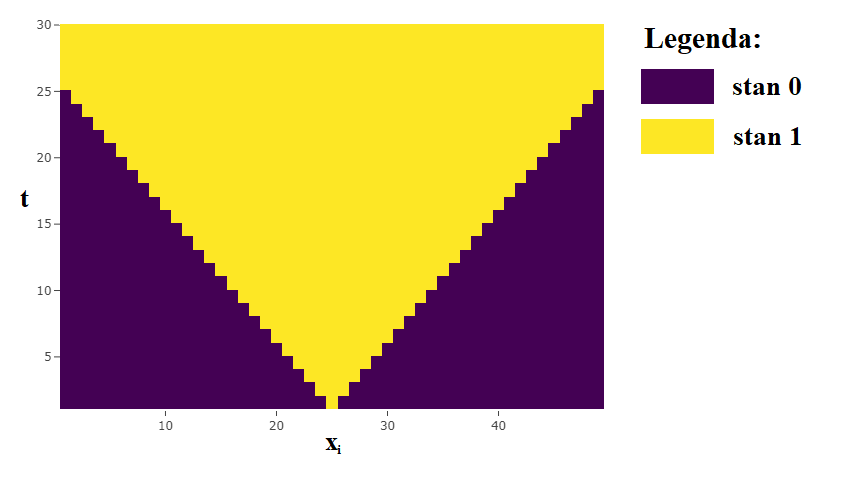
\includegraphics[width=7cm]{rule254.png}
    \caption{Zasada 254 z jedną chorą komórką na początku}
    \label{fig:my_label}
\end{figure}
\begin{figure}[h]
    \centering
    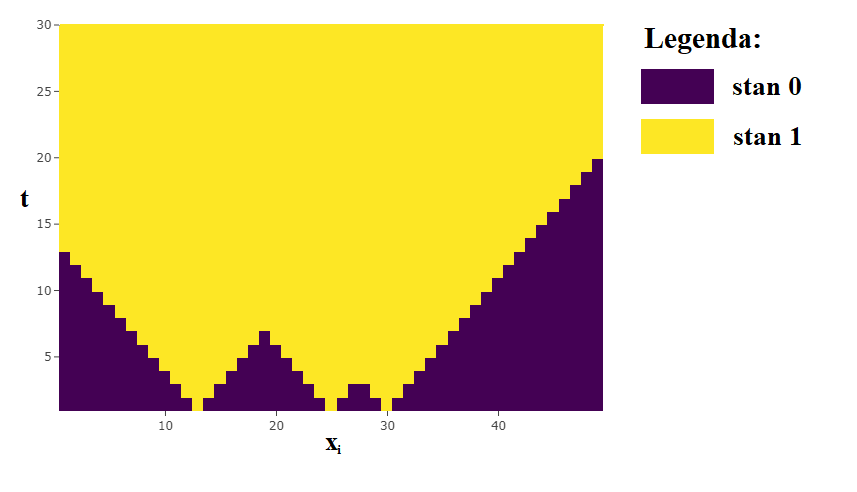
\includegraphics[width=7cm]{rule254l.png}
    \caption{Zasada 254 z kilkoma chorymi komórkami na początku}
    \label{fig:my_label}
\end{figure}
\\
Rysunki 2 oraz 3 przedstawiają, to jak rozprzestrzenia się infekcja w momencie, gdy tylko jedna z komórek jest zainfekowana. Jak możemy zauważyć, wraz z upływem czasu choruje ich coraz więcej, do momentu aż wszystkie stają się chore. Niezależnie od stanu początkowego zawsze po czasie otrzymamy to samo, pomijając trywialny przypadek, w którym wszystkie komórki są zdrowe. Automat ten jest idealnym reprezentantem I klasy Wolframa.\\
\subsubsection{Zasada 50}
Reguła ta przedstawia model infekcji podobny do poprzedniego, z tą różnicą, że teraz dopuszczamy możliwość wyzdrowienia komórki w następnym kroku. Możemy myśleć tu na przykład o przeziębieniu, w pierwszym tygodniu jesteśmy zdrowi, ale spotykamy chorego sąsiada, drugi tydzień chorujemy, a w trzecim udaje się nam dojść do siebie. W tym modelu:
$$
f(\tau(,t)|_{U(x_i)})= \left\{ \begin{array}{ll}
1 & \textrm{gdy $s\geq1$ oraz $\tau(x_i)=0,$}\\
0 & \textrm{w przeciwnym przypadku.}\\
\end{array} \right.
$$
Niezależnie z jakiej konfiguracji rozpoczniemy, to nasz obszar będzie się zmieniał okresowo. Każda komórka, która była w stanie 0, w następnym kroku przejdzie do stanu 1 i na odwrót, co można zaobserwować na rysunkach 4 oraz 5. Automat ten jest klasyfikowany w II klasie.
\begin{figure}[h]
\centering
    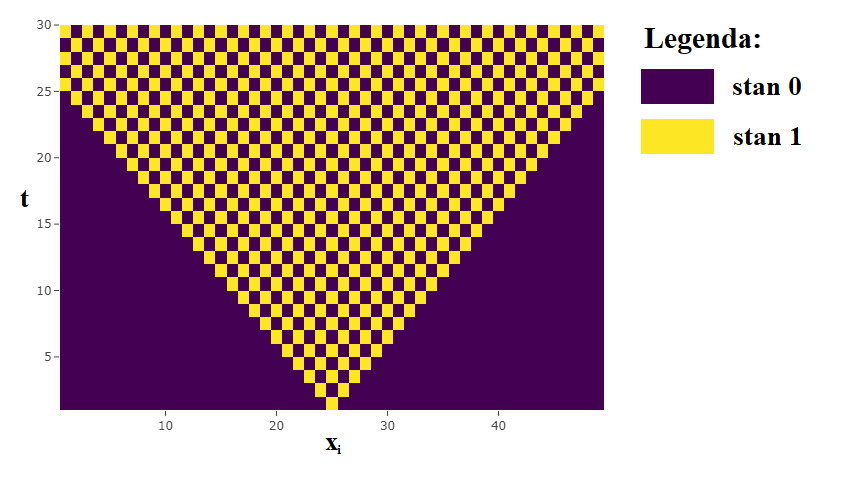
\includegraphics[width=7cm]{rule50.png}
    \caption{Zasada 50 z jedną chorą komórką na początku}
    \label{fig:my_label}
\end{figure}
\clearpage
\begin{figure}[h]
    \centering
    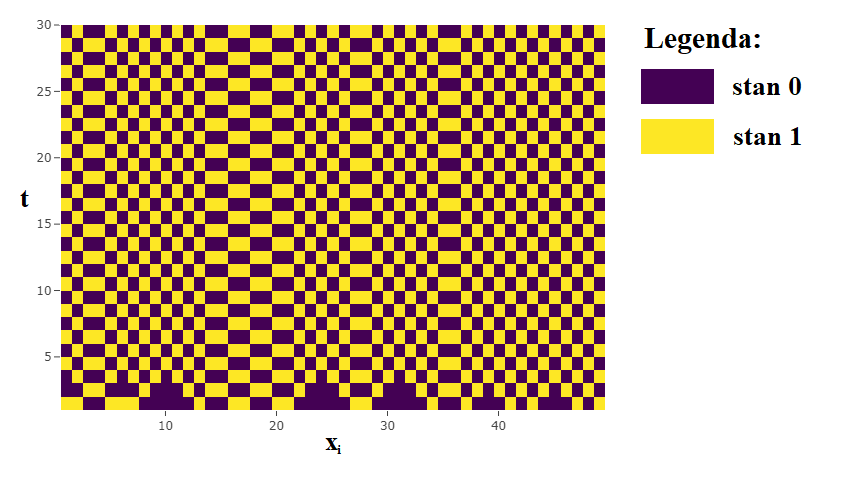
\includegraphics[width=7cm]{rule50l.png}
    \caption{Zasada 50 z kilkoma chorymi komórkami na początku}
    \label{fig:my_label}
\end{figure}

\subsubsection{Zasada 90}

Przejście komórek w zależności od sąsiedztwa, dla reguły 90, dobrze opisuje tabela 1. Tworząc symulacje zauważyłam, że funkcję, która opisuje te przejścia można zapisać wzorem: 
$$
f(\tau(,t)|_{U(x_i)})= \left\{ \begin{array}{ll}
1 & \textrm{gdy ($s=1$ i $\tau(x_i)=0$) lub ($s=2$ i $\tau(x_i)=1$)}\\
0 & \textrm{w przeciwnym przypadku.}\\
\end{array} \right.
$$

Gdy na początku tylko jedna komórka znajduje się w stanie 1, to po krótkiej obserwacji zmian możemy spróbować przewidzieć jak będzie się zmieniać układ w czasie. W momencie gdy w stanie początkowym infekcja dotyczy większej liczby komórek, to nie jest to już takie proste zadanie, wzór wyłania się bardziej chaotycznie. Automat jest przykładem należącym do III klasy.

\begin{figure}[h]
    \centering
    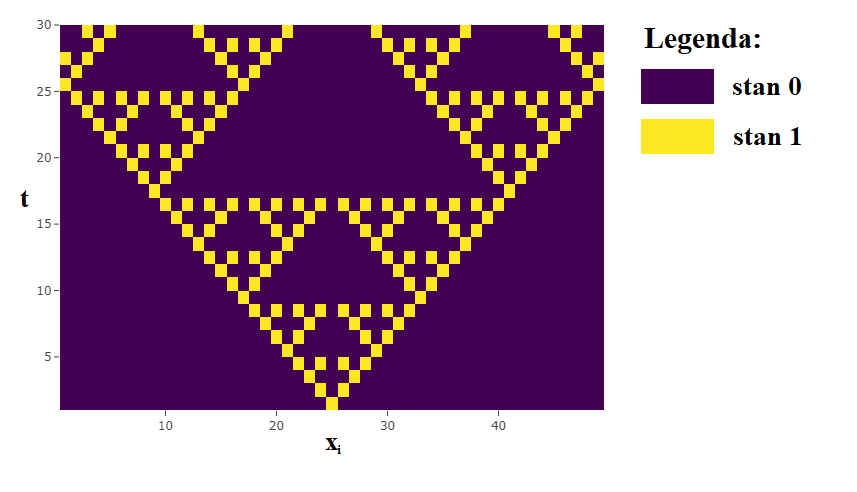
\includegraphics[width=7cm]{rule90.png}
    \caption{Zasada 90 z jedną chorą komórką na początku}
    \label{fig:my_label}
\end{figure}
\begin{figure}[h]
    \centering
    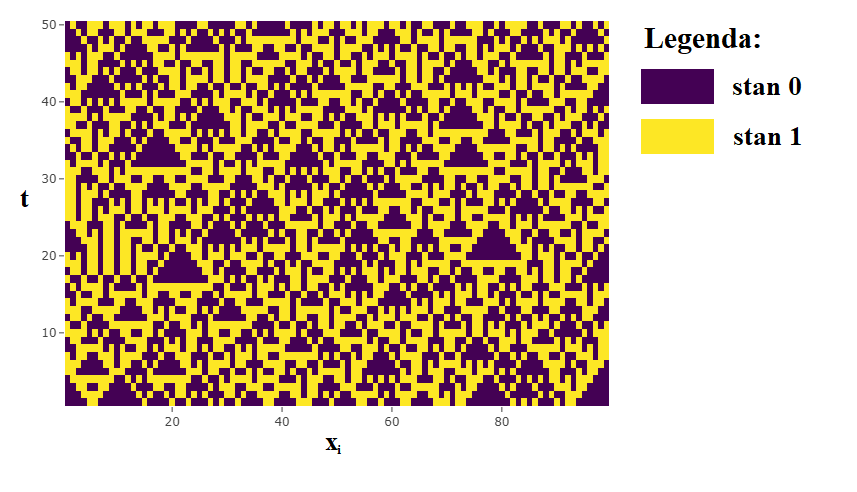
\includegraphics[width=7cm]{rule90l.png}
    \caption{Zasada 90 z kilkoma chorymi komórkami na początku}
    \label{fig:my_label}
\end{figure}
\newpage
\section{Znane przykłady automatów komórkowych na płaszczyźnie}

Wraz z rozpowszechnieniem się nowej dziedziny stworzonej przez von Neumann'a rozpoczęto pracę nad nowym sposobem tworzenia modeli. Jedną z osób, która wykorzystywała automaty komórkowe przy pracy był C. Langton, znany z badań nad sztucznym życiem\cite{lan}.\\
Wyróżniamy automat zwany pętlą Langton'a, który jest uproszczoną wersją pierwszego automatu komórkowego. Wykazuje ona mniejszą złożoność obliczeniową w porównaniu z już uproszczonym automatem, zaprezentowanym w 1968 roku przez E. F. Codd'a \cite{loop}. Poza redukcją liczby stanów z 29 na 8, jak to zrobił Codd, położono mniejszy nacisk na aspekt dotyczący uniwersalności. W tej pracy chciałam jednak zaprezentować inny automat, zaprojektowany przez tego amerykańskiego informatyka, zwany mrówką Langton'a.

\subsection{Mrówka Langton'a}
Mrówka Langton'a jest to dwuwymiarowy automat komórkowy z sąsiedztwem von Neumanna. Zasada działania jest dość prosta i polega ona na tym, że:
\begin{enumerate}
    \item Jeżeli mrówka stanie na komórce o stanie równym 0, to w następnym kroku skręca ona w lewo, a pole na którym stała zmienia stan na 1.
    \item Jeżeli mrówka stanie na komórce będącej w stanie 1, to skręca w prawo, a pole zmienia stan na 0.
\end{enumerate}
  Określenia lewo/prawo odnoszą się do kierunków postrzeganych przez mrówkę, więc to jak ona się porusza nie zależy tylko od stanu komórki, na którą stanie, ale również od tego, z której strony na dane pole weszła. Przykładowo, jeżeli mrówka stoi na komórce $x_{i-1j}$ i przechodzi na komórkę $x_{ij}$, to w następnym kroku pójdzie, w zależności od tego jaki stan przyjmowała komórka,  albo (w lewo) na $x_{ij+1}$, albo (w prawo) na $x_{ij-1}$. Taka instrukcja mogłaby wyglądać następująco:
\begin{verbatim}
#1. Mrówka przyszła z lewej strony, na komórkę w stanie 0. Przechodzi do góry,
    a komórka zmienia stan na 1.
      
      if( (Mr[y, x, t] == 2 ) & (Mr[y, x-1, t-1] == 2) 
            & (Mr[y, x, t-1] == 0) ){
            
        Mr[y+1, x, t+1] = 2
        Mr[y, x, t+1] = 1 
        Mr[y-1, x, t+1] = Mr[y-1, x, t] 
        Mr[y, x+1, t+1] = Mr[y, x+1, t] 
        Mr[y, x-1, t+1] = Mr[y, x-1, t] }
        
#2. Mrówka przyszła z lewej strony na komórkę w stanie 1. Przechodzi w dól,
    a komórka zmienia stan na 0.
      
      if( (Mr[y, x, t] == 2) & (Mr[y, x-1, t-1] == 2) 
            & (Mr[y, x, t-1] == 1) ){
            
        Mr[y-1, x, t+1] = 2
        Mr[y, x, t+1] = 0
        Mr[y+1, x, t+1] = Mr[y+1, x, t] 
        Mr[y, x+1, t+1] = Mr[y, x+1, t] 
        Mr[y, x-1, t+1] = Mr[y, x-1, t] }
\end{verbatim}
Zamieszczony fragment kodu był pisany w \verb R , przy użyciu programu \verb"RStudio", a przedstawiona instrukcja w całości umieszczona jest w dodatku na końcu pracy licencjackiej, w rozdziale 7.2.1. W przygotowanym przeze mnie programie możemy wyróżnić trzy stany, w jakich może znaleźć się komórka:
\begin{itemize}
    \item 0 - zaznaczony kolorem kremowym,
    \item 1 - zaznaczony kolorem jasnozielonym, 
    \item 2 - zaznaczony kolorem ciemnozielonym, oznacza aktualną pozycję w jakiej znajduje się mrówka;
\end{itemize} \\
Dzięki przeprowadzonym symulacjom możemy zaobserwować, to jak zachowuje się nasza mrówka w czasie. Na początek wybrałam pierwsze siedem kroków, dla nich wybrałam mniejszą kratę, abyśmy mogli dokładnie przyjrzeć się temu, jak działają zasady według, których mrówka się porusza. 
Dodatkowo naniosłam grafikę symbolizującą mrówkę, aby lepiej było widać kierunek, w którym właśnie podąża, a także gdzie może skręcić w następnym kroku.\\
\begin{figure}[!htb]
\centering
\subfloat[$t=1$]{\label{odnosnik}
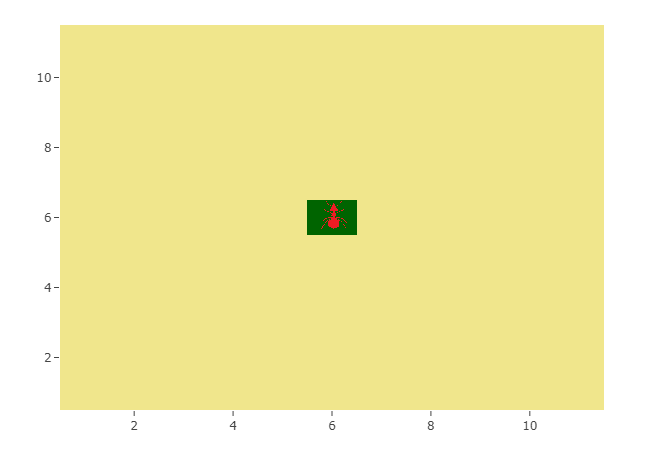
\includegraphics[width=0.3\textwidth]{mrt1.png}}
\quad
\subfloat[$t=2$]{\label{odnosnik}
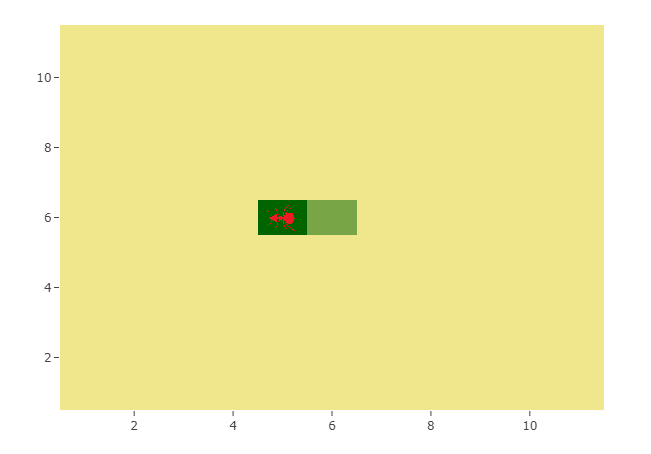
\includegraphics[width=0.3\textwidth]{mrt2.png}}
\quad
\subfloat[$t=3$]{\label{odnosnik}
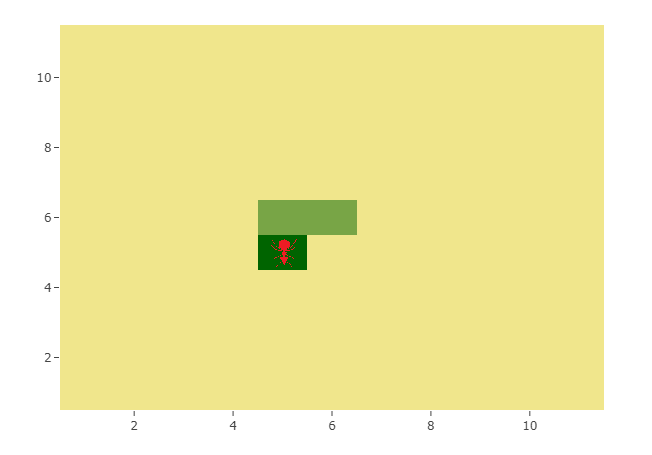
\includegraphics[width=0.3\textwidth]{mrt3.png}}
\quad
\subfloat[$t=4$]{\label{odnosnik}
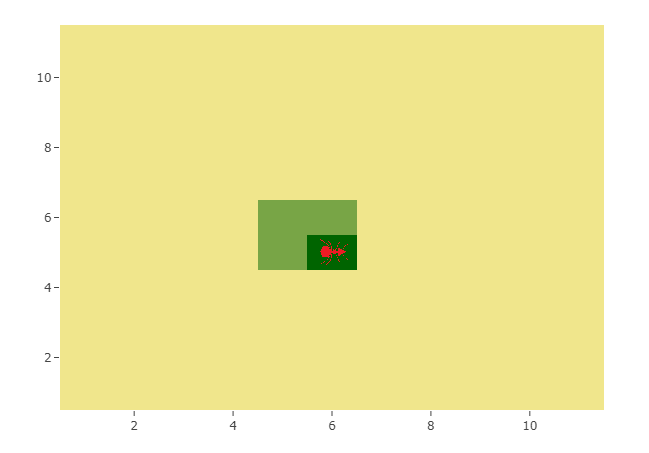
\includegraphics[width=0.3\textwidth]{mrt4.png}}
\quad
\subfloat[$t=5$]{\label{odnosnik}
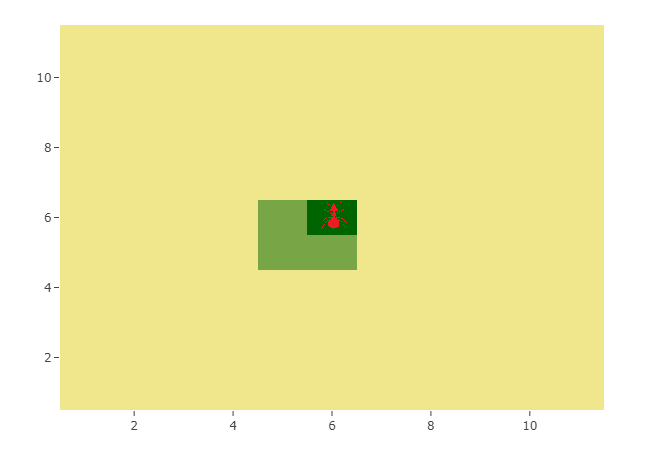
\includegraphics[width=0.3\textwidth]{mrt5.png}}
\quad
\subfloat[$t=6$]{\label{odnosnik}
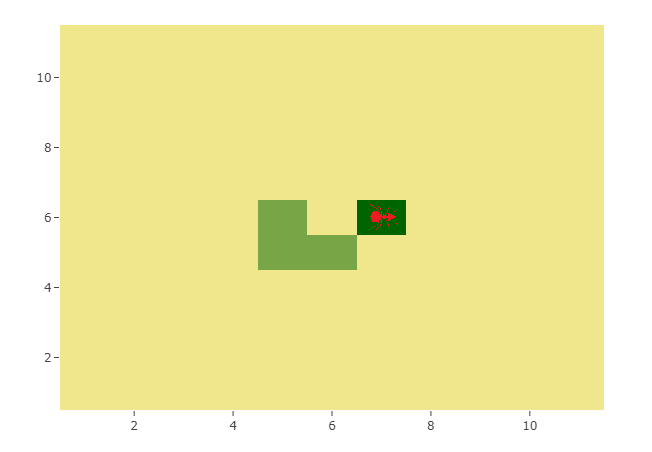
\includegraphics[width=0.3\textwidth]{mrt6.png}}
\quad
\subfloat[$t=7$]{\label{odnosnik}
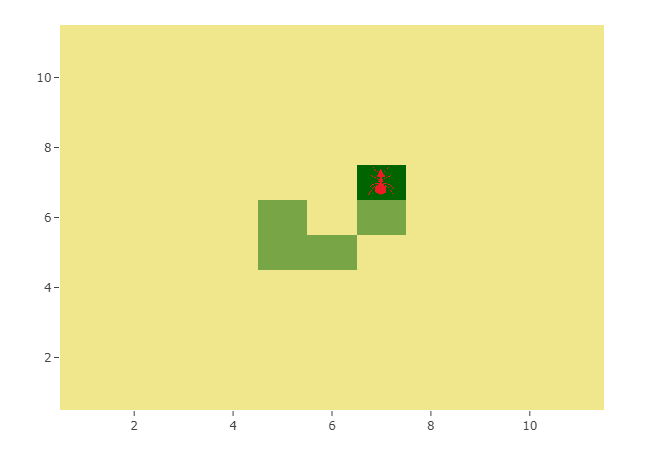
\includegraphics[width=0.3\textwidth]{mrt7.png}}
\caption{Kroki mrówki Langton'a}
\label{fig:animals}
\end{figure}

Początkowe kroki układają się symetrycznie, a odległości od miejsca, w którym rozpoczynaliśmy spacer są niewielkie. 
Wraz z upływem czasu tworzą się coraz bardziej chaotyczne wzory i utrzymują się one do około $10 000$ kroku \cite{l}.
\begin{enumerate}
    \item Symetryczne wzory (Rysunek 9)
\begin{figure}[!htb]
\centering
\subfloat[$t=100$]{\label{odnosnik}

\includegraphics[width=0.25\textwidth]{mrt100zoom.png}}
\quad
\subfloat[$t=200$]{\label{odnosnik}

\includegraphics[width=0.25\textwidth]{mrt200zoom.png}}
\quad
\subfloat[$t=500$]{\label{odnosnik}
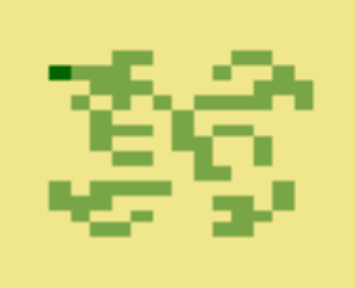
\includegraphics[width=0.25\textwidth]{mrt500xoom.png}}
\caption{Symetryczne wzory mrówki Langton'a w przybliżeniu}
\label{fig:animals}
\end{figure}    
\item Chaotyczne wzory (Rysunek 10)
\begin{figure}[!htb]
\centering
\subfloat[$t=1000$]{\label{odnosnik}
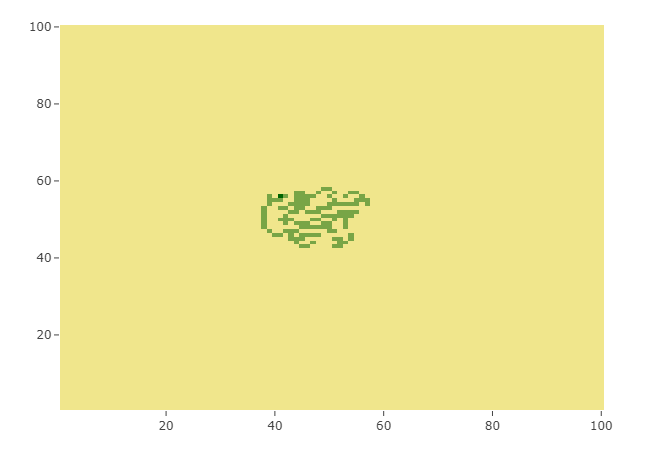
\includegraphics[width=0.3\textwidth]{mrt1000.png}}
\quad
\subfloat[$t=10000$]{\label{odnosnik}
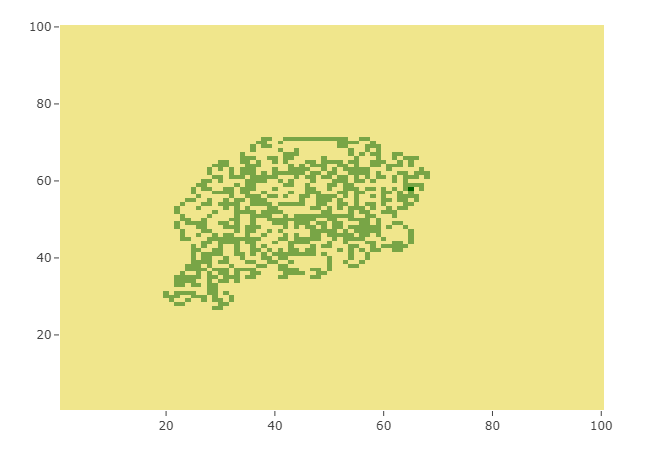
\includegraphics[width=0.3\textwidth]{mrt10000.png}}
\quad
\subfloat[$t=10200$]{\label{odnosnik}
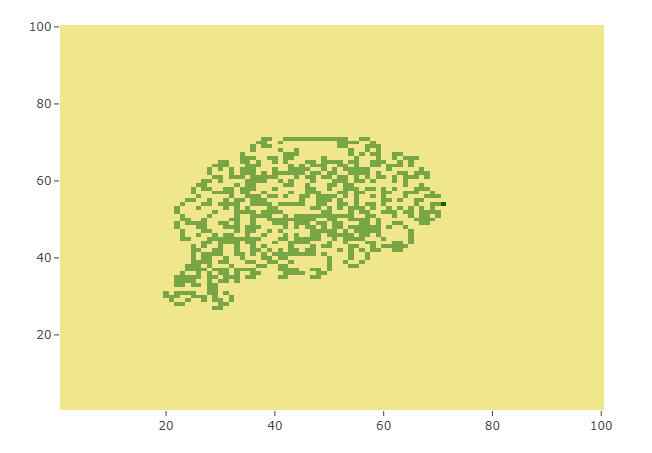
\includegraphics[width=0.3\textwidth]{mrt10200.png}}
\caption{Chaotyczne wzory mrówki Langton'a}
\label{fig:animals}
\end{figure}
\item Około kroku 10300 zaczyna wyłaniać się symetryczny fragment. Mrówka kieruje się autostradą w jednym kierunku. (Rysunek 11)
\begin{figure}[!htb]
\centering
\subfloat[$t=10300$]{\label{odnosnik}
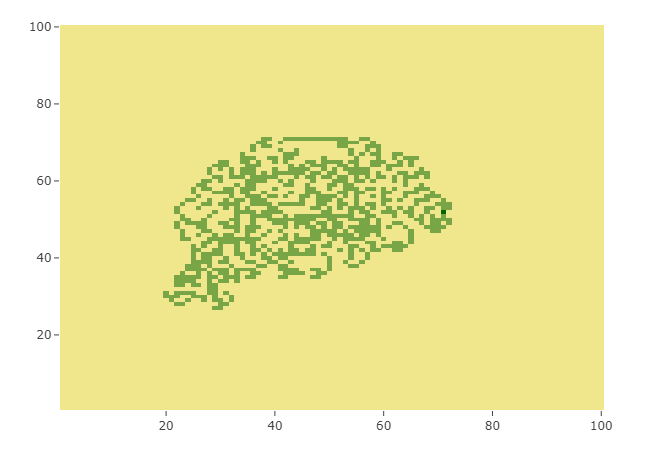
\includegraphics[width=0.3\textwidth]{mrt10300.png}}
\quad
\subfloat[$t=10500$]{\label{odnosnik}
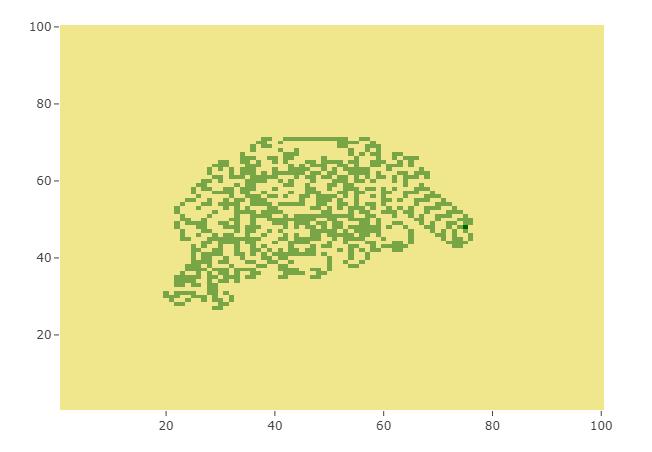
\includegraphics[width=0.3\textwidth]{mrt10500.png}}
\quad
\subfloat[$t=10200$]{\label{odnosnik}
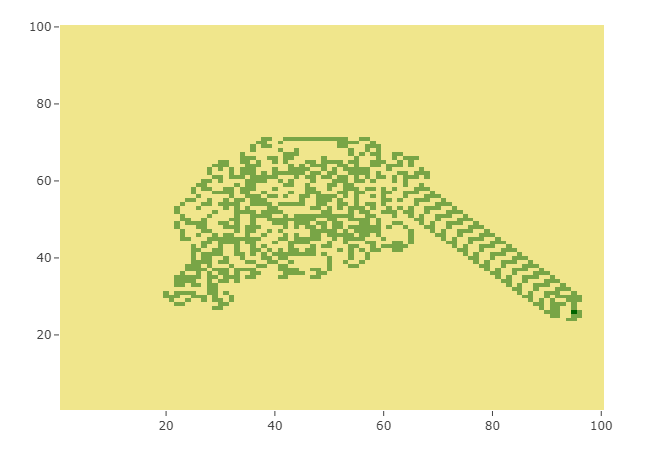
\includegraphics[width=0.3\textwidth]{mrt11500.png}}
\caption{Autostrada mrówki Langton'a}
\label{fig:animals}
\end{figure}
\end{enumerate}
\newpage
Ciekawe jest to, że niezależnie jakie warunki początkowe zadamy, to mrówka prędzej czy później, zacznie podążać autostradą. Istnieje przypuszczenie, że autostrada ta jest atraktorem mrówki, ale sprawa ta nadal pozostaje nierozstrzygnięta (Rysunek 11)\cite{l}.
Mrówka to uniwersalna maszyna Turinga, oparta na zbiorze prostych reguł. Jej uniwersalność udowodniono w 2000 roku \cite{200}. Automat ten był również przerabiany i uogólniany na większą liczbę stanów/kolorów.
\newpage
\subsection{"Gra w życie" Conway'a}

"Gra w życie" jest to najpopularniejszy automat, z jakim możemy się spotkać. Jego twórca J. Conway był jednym z pionierów nowo powstałej dziedziny, a jego automat komórkowy zapoczątkował  nową erę, jeżeli chodzi o symulacje komputerowe \cite{hill}. Słowo gra jest użyte raczej symbolicznie, ponieważ wkład użytkownika w jej przebieg ogranicza się do ustalenia stanu początkowego, z którego automat będzie mógł wystartować i dalej samodzielnie ewoluować, na podstawie zadanych i ustalonych zasad. \\
Reguły jakie rządzą w tym automacie są dość proste i imitują zachowania, jakie możemy zaobserwować w naturze, wśród zwierząt i roślin, takie jak konkurencja. Zasady te można opisać następującym wzorem:\\
$$
f(\tau(,t)|_{U(x_{ij})})= \left\{ \begin{array}{ll}
1 & \textrm{gdy $s=3,$}\\
1 & \textrm{gdy $s=2$ oraz $\tau(x_{ij})=1$},\\
0 & \textrm{w przeciwnym przypadku,}\\
\end{array} \right.
$$
gdzie $s$ oznacza suma stanów wszystkich komórek należących do sąsiedztwa $x_{ij}$, włącznie z ${x_{ij}}$ \cite{hill}. Reguły te mają przełożenie, gdy rozważamy nieskończoną kratę. 
Na potrzeby symulacji dobrałam do nich warunki brzegowe, odpowiednio przeskalowane, w stosunku do oryginalnych zasad. Wyglądają one następująco:
\begin{itemize}
    \item Jeżeli $x_{ij}$ należy do brzegu, ale nie leży na rogu:
    $$
f(\tau(,t)|_{U(x_{ij})})= \left\{ \begin{array}{ll}
1 & \textrm{gdy $s=2,$}\\
1 & \textrm{gdy $s=1$ oraz $\tau(x_{ij})=1$},\\
0 & \textrm{w przeciwnym przypadku,}\\
\end{array} \right.
$$
\item Jeżeli $x_{ij}$ leży na jednym  czterech rogów siatki:
$$
f(\tau(,t)|_{U(x_{ij})})= \left\{ \begin{array}{ll}
1 & \textrm{gdy $s=1,$}\\
1 & \textrm{gdy $s=0$ oraz $\tau(x_{ij})=1$},\\
0 & \textrm{w przeciwnym przypadku.}\\
\end{array} \right.
$$
\end{itemize}
Jest to przykład dwuwymiarowego automatu należącego do IV klasy Wolframa \cite{hill}. Ustalając warunki początkowe nie mamy żadnej pewności, jaki wzór uzyskamy, co więcej przez długi czas wzór jaki obserwujemy jest chaotyczny i wygląda tak, jakby miał taki pozostać. Dopiero po upływie dłuższego czasu zaczynają wyłaniać się symetryczne i okresowe wzory.  Rysunek 12 przedstawia efekty działania "Gry w życie", dla układu z losowo dobranym stanem początkowym, na kracie o wymiarach $100$x$100$. Kolor kremowy reprezentuje stan 0, natomiast zielony 1. 
\begin{figure}[!htb]
\centering
\subfloat[Stan początkowy, $t=1$]{\label{odnosnik}
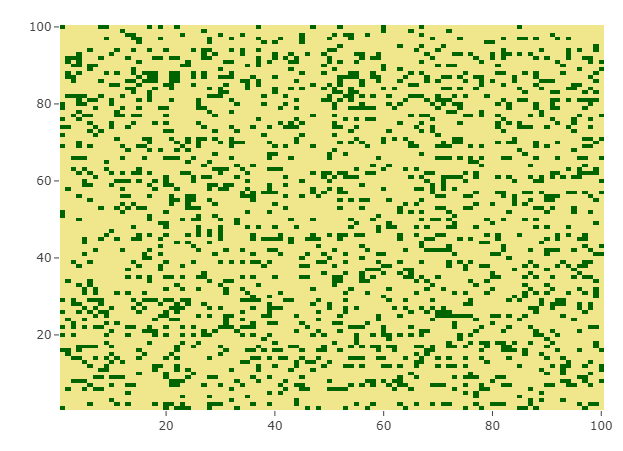
\includegraphics[width=0.3\textwidth]{tab_m_g_t1.png}}
\quad
\subfloat[Pierwsze przejście komórek do nowych stanów, $t=2$]{\label{odnosnik}
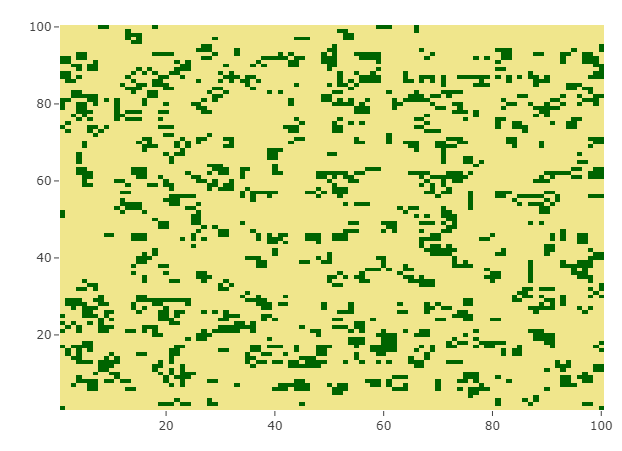
\includegraphics[width=0.3\textwidth]{tab_m_g_t2.png}}
\quad
\subfloat[Wyłanianie się pierwszych wzorów i powolna stabilizacja układu, $t=50$]{\label{odnosnik}
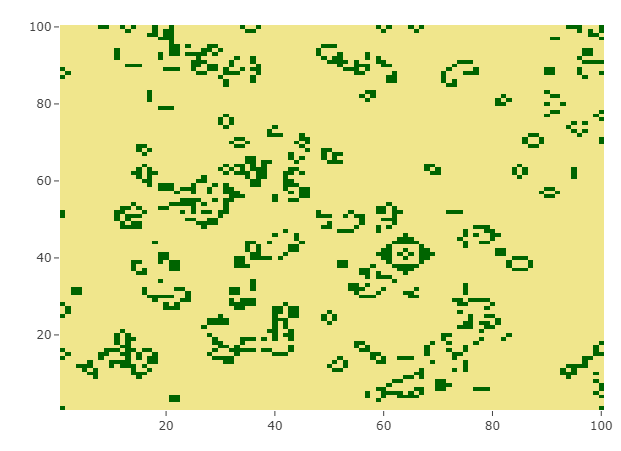
\includegraphics[width=0.3\textwidth]{tab_m_g_t50.png}}
\quad
\subfloat[Układ stabilny, w którym możemy wyróżnić wzory  stałe i oscylujące, $t=425$]{\label{odnosnik}
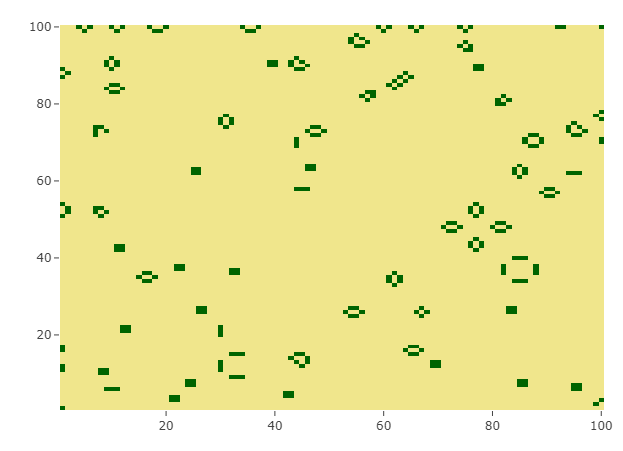
\includegraphics[width=0.3\textwidth]{tab_m_g_t425.png}}
\quad
\subfloat[Układ stabilny, widoczna zmiana przy wzorach oscylujących, $t=426$]{\label{odnosnik}
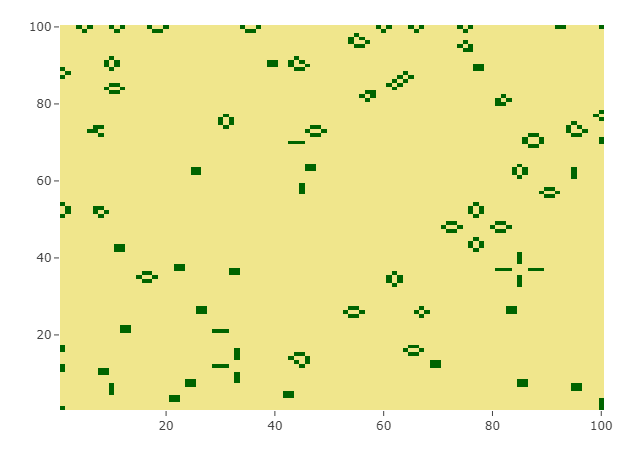
\includegraphics[width=0.3\textwidth]{tab_m_g_t426.png}}
\quad
\subfloat[Układ stabilny, identyczny jak w kroku 425, $t=427$]{\label{odnosnik}
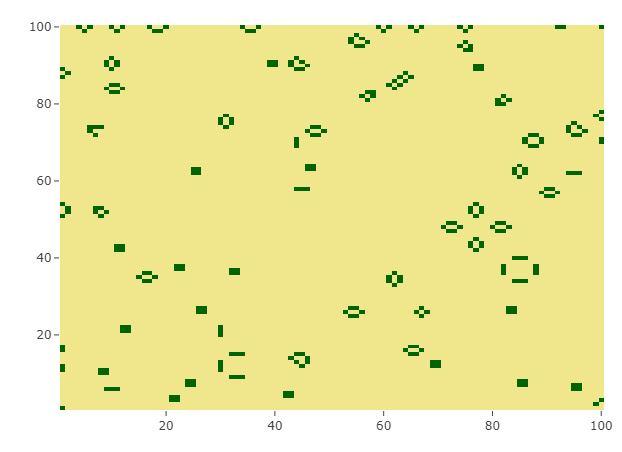
\includegraphics[width=0.3\textwidth]{tab_m_g_t427.png}}
\caption{Ewolucja w Grze w życie}
\label{fig:animals}
\end{figure}

W "Grze w życie" wzory, które się tworzą możemy sklasyfikować pod względem tego, jak zachowują się wraz z upływem czasu. Rozpoznajemy wzory stałe, które gdy się uformują, to pozostaną niezmienne w czasie, przykład takich wzorów pokazany jest na rysunku 13c. Drugi rodzaj to wzory oscylujące, ale bez zmiany pozycji, w której się znajdują, co mogliśmy dostrzec na  powyższej symulacji i na rysunku 14 \cite{o}. Trzecim elementem z tej rodziny są struktury, które się przemieszczają np. "statki kosmiczne" z rysunkach 13a i 13b \cite{st}.
Ostatnimi i najciekawszymi są wzory odkryte w roku 2015 (i później), mianowicie takie, które rozwijają się w nieskończoność, przykład takiej struktury i kilka kroków pokazałam na rysunku 15 \cite{2015}.
\begin{figure}
\centering
\subfloat[Struktury ruchome, \\$t=1$]{\label{odnosnik}
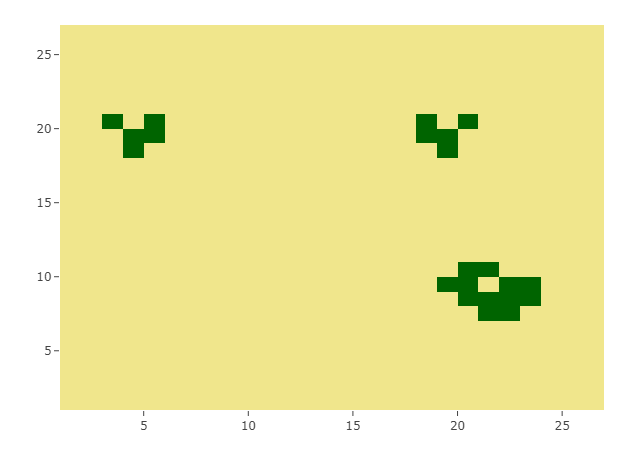
\includegraphics[width=0.3\textwidth]{statki1.png}}
\quad
\subfloat[Struktury ruchome, \\$t=11$]{\label{odnosnik}
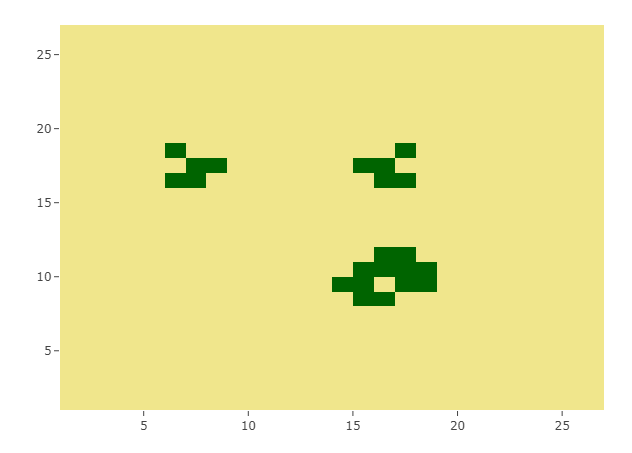
\includegraphics[width=0.3\textwidth]{statki11.png}}
\quad
\subfloat[Struktury stałe, które powstały po "zderzeniu" statków z rysunku ... i ustabilizowaniu się wzoru, \\$t=45$]{\label{odnosnik}
\includegraphics[width=0.3\textwidth]{statki45(stałe).png}}
\caption{Struktury stałe i ruchome}
\label{fig:animals}
\end{figure}

\begin{figure}
\centering
\subfloat[$t=1$]{\label{odnosnik}
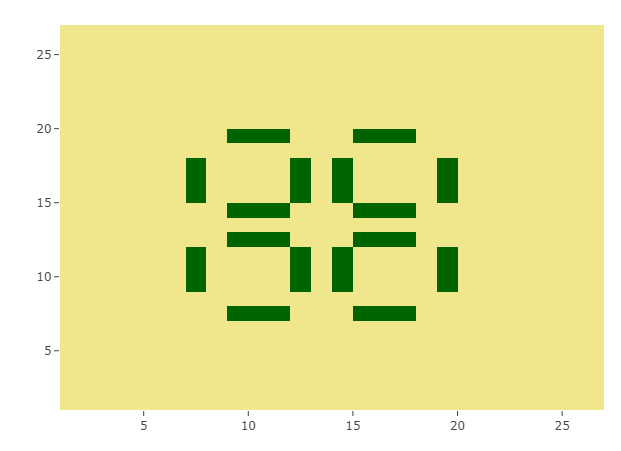
\includegraphics[width=0.3\textwidth]{pulser1.png}}
\quad
\subfloat[$t=2$]{\label{odnosnik}
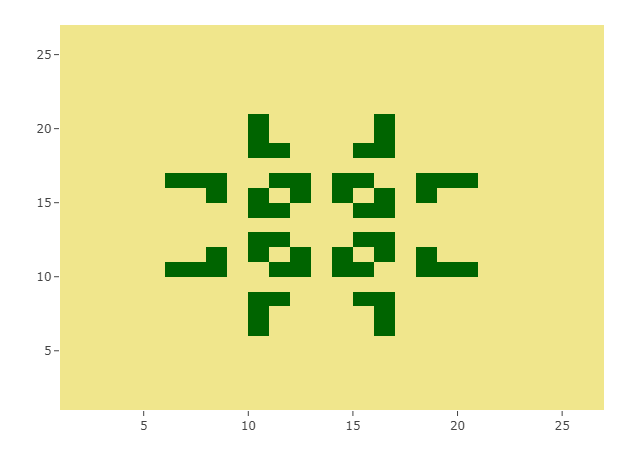
\includegraphics[width=0.3\textwidth]{pulser2.png}}
\quad
\subfloat[$t=3$]{\label{odnosnik}
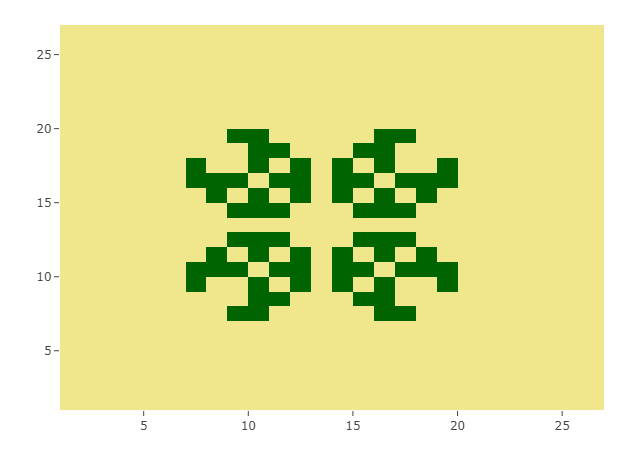
\includegraphics[width=0.3\textwidth]{pulser3.png}}
\caption{Przykład wzoru pulsującego (okres = 3)}
\label{fig:animals}
\end{figure}

\begin{figure}
\centering
\subfloat[$t=1$]{\label{odnosnik}
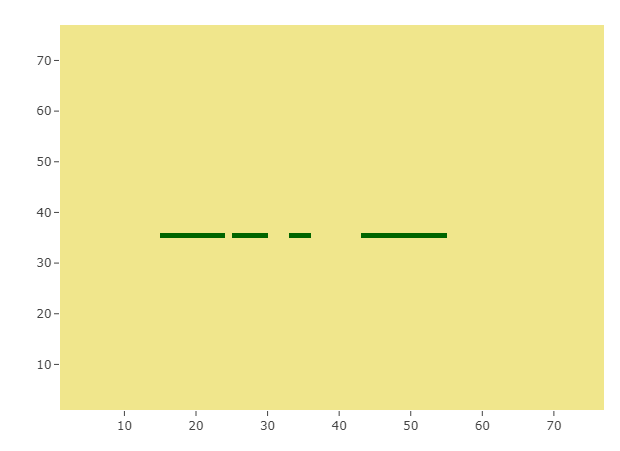
\includegraphics[width=0.3\textwidth]{pasy1.png}}
\quad
\subfloat[$t=10$]{\label{odnosnik}
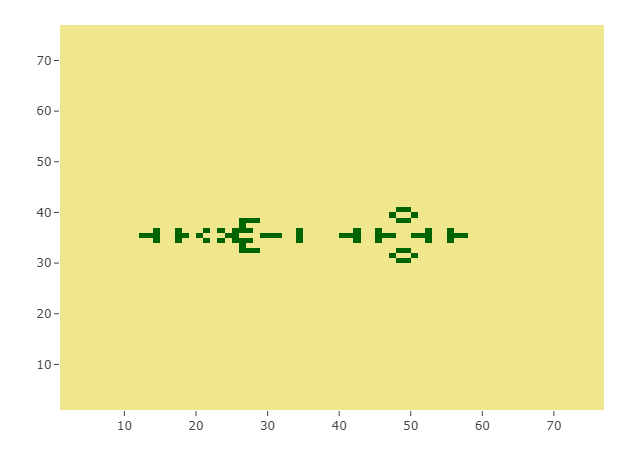
\includegraphics[width=0.3\textwidth]{pasy10.png}}
\quad
\subfloat[$t=50$]{\label{odnosnik}
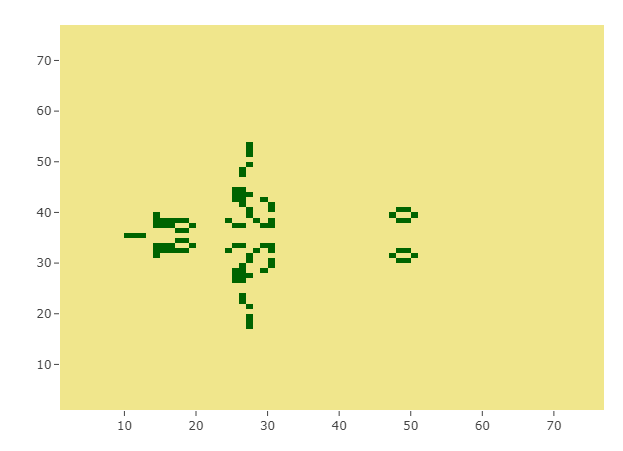
\includegraphics[width=0.3\textwidth]{pasy50.png}}
\caption{Przykład wzoru rozszerzającego się w nieskończoność}
\label{fig:animals}
\end{figure}
\clearpage

\section{Równanie dyfuzji}

Rozdział ten został tworzony na podstawie książki autorstwa Murry'a \cite{mb}.

\subsection{Równanie dyfuzji i prawo Ficka}

Dyfuzja to zjawisko, z którym każdy ma styczność w życiu codziennym, np. w kuchni podczas gotowania wody na makaron. Żeby lepiej zrozumieć na czym dokładnie polega i jakie procesy fizyko-chemiczne za nią stoją, wyobraźmy sobie, że mamy rurkę wypełnioną wodą zamkniętą z dwóch stron. Przez jeden z krańców rurki wpuszczamy pewną ilość barwnika (bez wylewania wody). Jak będziemy obserwować naszą rurkę zauważymy, że na początku barwnik koncentruje się przy końcu, przez który został dodany, aby z czasem rozchodzić się coraz dalej wgłąb rurki. Przechodzenie barwnika będzie trwać do momentu aż jego stężenie nie wyrówna się i cała woda w rurce nie wymiesza się z barwnikiem.     
\\
Załóżmy, że rurka ma początek w punkcie $a$, a koniec w punkcie $b$. Przez $M$ oznaczmy masę barwnika w rurce. Niech $u(x,t)$ oznacza koncentrację barwnika w punkcie $x$, w chwili $t$, czyli masę barwnika na jednostkę długości. Wtedy masę barwnika w rurce można opisać w następujący sposób:
\begin{equation}
    M(x)=\int_a^b u(x,t) dx 
\end{equation}
Prawo zachowania masy mówi, że ilość substancji w rurce może zmienić się wtedy i tylko wtedy, gdy wpłynie lub wypłynie przez brzeg. Matematycznie zapisuje się to jak:
$$\frac{\partial M(x)}{\partial t}= J(b) - J(a), $$
gdzie $J=Du_x$.
Z pierwszego prawa Ficka mamy, że prędkość z jaką barwnik przechodzi z jednego obszaru do drugiego jest proporcjonalna do gradientu koncentracji. Zatem zmiany w ilości barwnika w zależności od czasu możemy zapisać jako:
\begin{equation}
    \frac{\partial M(x)}{\partial t}= D\Big(u_x(b,t)-u_x(a,t)\Big),
\end{equation}
gdzie $D>0$ oznacza stałą proporcjonalności.
Z równania (2) otrzymujemy:
$$ \int_a^b u_t(x,t) dx = D\int_a^b u_{xx}(x,t)dx. $$ 
Zakładamy, że  $u$ jest dostatecznie regularną funkcją oraz ponieważ odcinek $[a,b]$ jest dowolny, dostajemy równanie dyfuzji.
\begin{equation}
    u_t(x,t)=Du_{xx}(x,t).
\end{equation}


\subsection{Wyprowadzenie równania dyfuzji za pomocą błądzenia losowego}

Rozważmy błądzenie losowe cząsteczki na prostej. Zasada, która mówi o tym jak cząsteczka będzie się poruszać będzie brzmieć następująco:\\\\
\textit {"Jeżeli cząsteczka w chwili $t_{k}$ znajduje się w komórce $x$, tzn. komórka $x_i$ przyjmuje wartość 1, to w kroku $t_{k+1}$, z prawdopodobieństwem $\frac{1}{2}$, znajdzie się ona w komórce $x_{i-1}$ lub z prawdopodobieństwem $\frac{1}{2}$ przejdzie do komórki $x_{i+1}$."}\\
Oznaczymy przez $u(x_i,t_k)$ prawdopodobieństwo, że cząsteczka znajdzie się w punkcie $x_i$ w czasie $t_k$. Wtedy model możemy opisać wzorem:
\begin{equation}
    u(x_i,t_{k+1})= \frac{ u(x_{i-1},t_k)+u(x_{i+1},t_k) }{2}.
\end{equation}
Aby móc manipulować wielkością komórek i długością kroku czasowego wprowadźmy dwie zmienne:

\begin{itemize}
    \item $\Delta x$ - długość komórek,
    \item $\Delta t$ - długość jednego kroku.
\end{itemize}

Wtedy $x_{i+1}=x_i+\Delta x$, a $t_{k+1}=t_{k}+\Delta t$, więc wzór (1) przyjmie postać
\begin{equation}
    u(x_i,t_k+\Delta t)= \frac{ u(x_{i}-\Delta x,t_k)+u(x_{i}+\Delta x,t_k) }{2}. 
\end{equation}

\begin{tw}
Załóżmy, że $u(x, t)$ jest dwa razy różniczkowalne w sposób ciągły względem $x$ i raz różniczkowalne względem $t$. Oznaczmy $D=\frac{(\Delta x)^2}{2\Delta t}>0$ i przyjmijmy, że jest to stała. Wtedy dla  $\Delta x \rightarrow 0$, $\Delta t \rightarrow 0$, równanie (5) redukuje się do równania dyfuzji $u_t(x,t)=Du_{xx}(x,t)$.

\end{tw}
\\
\textbf{Dowód}\\

Ustalmy $x_i\in\mathbb{R}$ i $t_k>0$. Równanie (5) możemy zapisać w sposób równoważny jako
$$  \frac{u(x_i,t_k+\Delta t) - u(x_i, t_k)}{\Delta t} = D\frac{u(x_i-\Delta x,t_k) + u(x_i+\Delta x, t_k)-2u(x_i,t_k)}{(\Delta x)^2}, $$
gdzie $D=\frac{\Delta t}{2(\Delta x)^2}.$
Możemy zauważyć, że gdy skorzystamy z założenia, że  $\Delta t \rightarrow 0$ otrzymamy
$$\lim_{\Delta t \rightarrow 0}\frac{u(x_i,t_k+\Delta t) - u(x_i, t_k)}{\Delta t}=u_t(x_i,t_k),$$
z definicji pochodnej.\\
Aby udowodnić, że prawa strona równania zbiega do $Du_{xx}$, przy $\Delta x\rightarrow 0$ skorzystamy ze wzoru Taylora, który wygląda następująco:
$$f(x+h)=f(x)+f'(x)h+u''(x)\frac{h^2}{2}+R(x,h),$$
przy założeniu, że
$$\lim_{h\rightarrow 0}\frac{R(x,h)}{h^2}=0.$$
Rozpisujemy składowe zgodnie ze wzorem
$$u(x_i-\Delta x,t_k) = u(x_i,t_k)-u_x(x_i,t_k)\Delta x+u_{xx}(x_i,t_k)\frac{(\Delta x)^2}{2}+R_1(x,h),$$
$$u(x_i+\Delta x,t_k) = u(x_i,t_k)+u_x(x_i,t_k)\Delta x+u_{xx}(x_i,t_k)\frac{(\Delta x)^2}{2}+R_2(x,h).$$
Jeżeli przejdziemy z prawą stroną równania do granicy, przy $\Delta x\rightarrow0$ i skorzystamy ze wzorów Taylora otrzymamy:
$$\lim_{\Delta x\rightarrow0}D\frac{u_{xx}(x_i,t_k)(\Delta x)^2+R_1(x,\Delta x)+R_2(x,\Delta x)}{(\Delta x)^2}=Du_{xx}(x_i,t_k).$$ 
Dzięki czemu otrzymujemy równanie dyfuzji
\begin{equation}
u_t(x_i,t_k)=Du_{xx}(x_i,t_k),
\end{equation}
co kończy dowód twierdzenia 1.
\subsection{Automat komórkowy w równaniu dyfuzji}

Wykorzystamy wzór (4) by zdefiniować automat komórkowy postaci \\ $A=(G,E,U,f)$ dla równania dyfuzji (9). Korzystamy z oznaczeń wprowadzonych w rozdziale 2. Niech
\begin{itemize}
    \item $G =\mathbb{Z}$ - jednowymiarowa siatka,
    \item $E = [0,1]$ - zbiór stanów,
    \item $U(x_i)= \{x_{i-1}, x_i,x_{x+1}\}$ - sąsiedztwo komórki $x_i$,
    \item $\tau(x_i,t_k)$ - stan komórki $x_i$ w kroku $t_k$,
    \item $f(\tau(\cdot,t)|_{U(x_i)})= \frac{\tau(x_{i + 1}, t_k)+\tau(x_{i-1},t_k) }{2}$ - funkcja przejścia.
\end{itemize}
Symulacje na podstawie powyższego automatu zostały przeprowadzone dla trzech zagadnień z różnymi warunkami brzegowymi. W związku z tym, że automat komórkowy został zaprojektowany dla nieskończonej przestrzeni, natomiast symulacje przeprowadzone zostały dla pewnego odcinka, należałoby wspomnieć o warunkach brzegowych i tym jak zostały one wprowadzane do programu. Będzie można o tym przeczytać przy każdym zagadnieniu (5.3.1-5.3.3) oraz obejrzeć w kodzie zamieszczonym w sekcjach 5.4 i 5.5. 
\subsubsection{Zagadnienie Dirichleta}
Przeprowadziłam symulację dla powyższego automatu, która pokazuje zachowanie dyfuzji na odcinku [0,1], z warunkiem początkowym postaci $$\tau(x,0)=\sin(\pi x)$$ i warunkami brzegowym Dirichleta $$x_0=x_n=0.$$ 
Przy powyższych warunkach jeden i drugi brzeg mają zawsze tą samą wartość równą zeru, niezależnie od tego co się dzieje z pozostałymi komórkami. Zostają one zdefiniowane na samym początku, tuż po deklaracji zmiennych, wyborze warunków początkowych i stworzeniu macierzy do której będą wpisywane dane z późniejszych wyliczeń. Podczas działania programu wartości na brzegu są uwzględniane, aby poprawnie uzupełnić sąsiednie komórki, ale same pozostają niezmienione. 
Zatem rozważamy zagadnienie 
\begin{equation}
    \begin{array}{llll}
    u_t(x,t)&=&u_{xx}(x,t),&x\in(0,1),\\
    u(x,0)&=&\sin\pi x,\\
    u(0,t)&=&u(1,t)=0, \end{array}
\end{equation}
którego rozwiązanie jest dane wzorem $$u(x,t) = e^{-\pi^2t}\sin\pi x.$$
Możemy zauważyć, że przy $t\rightarrow\infty$ rozwiązanie zagadanienia (7) zbiega do 0.
Wyobraźmy sobie, że nasz odcinek jest prętem, który na początku eksperymentu jest nierównomiernie ogrzany. Przy tych warunkach pręt z czasem będzie robił się coraz chłodniejszy.
\begin{figure}[!htb]
    \centering
    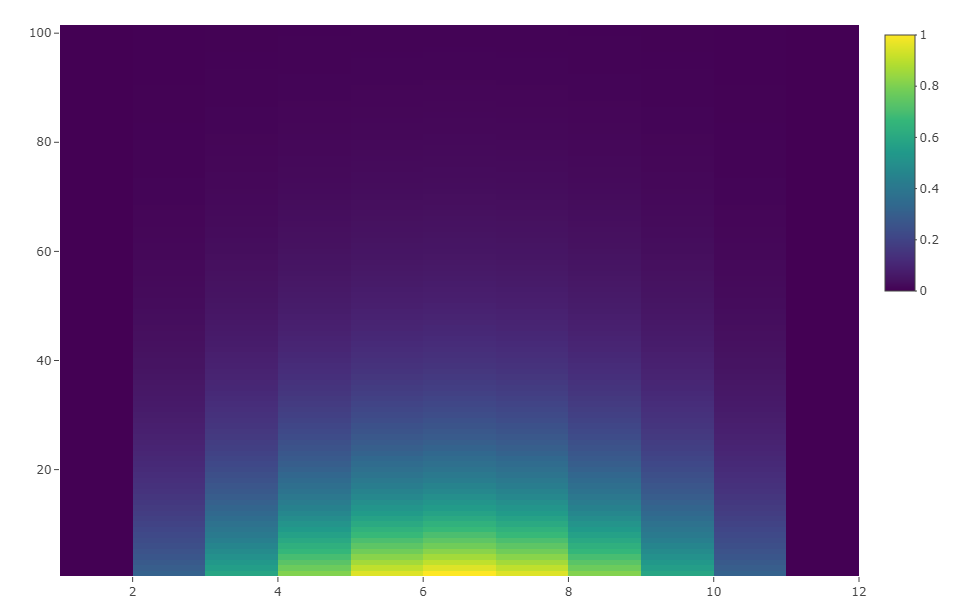
\includegraphics[width=6.5cm]{dyfuzaj.png}
    \caption{Dyfuzja na odcinku dla zagadnienia (7) z wykorzystaniem automatu komórkowego}
    \label{fig:my_label}
\end{figure}
\newpage
\subsubsection{Zagadnienie Neumanna}
 Warunki brzegowe dla tego zagadnienia warunkują brak przepływu przez brzeg. W automacie komórkowym komórka na brzegu przyjmuje wartość, która została wyliczona dla jej sąsiada. W odróżnieniu od poprzedniego zagadnienia dane dla komórek na brzegach wpisywane są w pętli, a nie jak wcześniej na początku całego programu.
 Zagadnienie z warunkami brzegowymi Neumanna wygląda następująco:
\begin{equation}
    \begin{array}{llll}
    u_t(x,t)&=&u_{xx}(x,t),&x\in(0,1),\\
    u(x,0)&=&\cos\pi x,\\
    u_x(0,t)&=&u_x(1,t)=0,
    \end{array}
\end{equation}
którego rozwiązanie jest dane jawnym wzorem $$u(x,t) = e^{-\pi^2t}\cos\pi x.$$
Rozwiązanie dla tego zagadnienia zbiega do 0. Jeżeli założymy, że nasz nasz odcinek symbolizuje pręt, który na początku jest odpowiednio rozgrzany, to przy warunkach brzegowych Neumanna, gdzie mamy brak przepływu przez brzeg, temperatura wyrówna się na długości całego odcinka.
\begin{figure}[!htb]
    \centering
    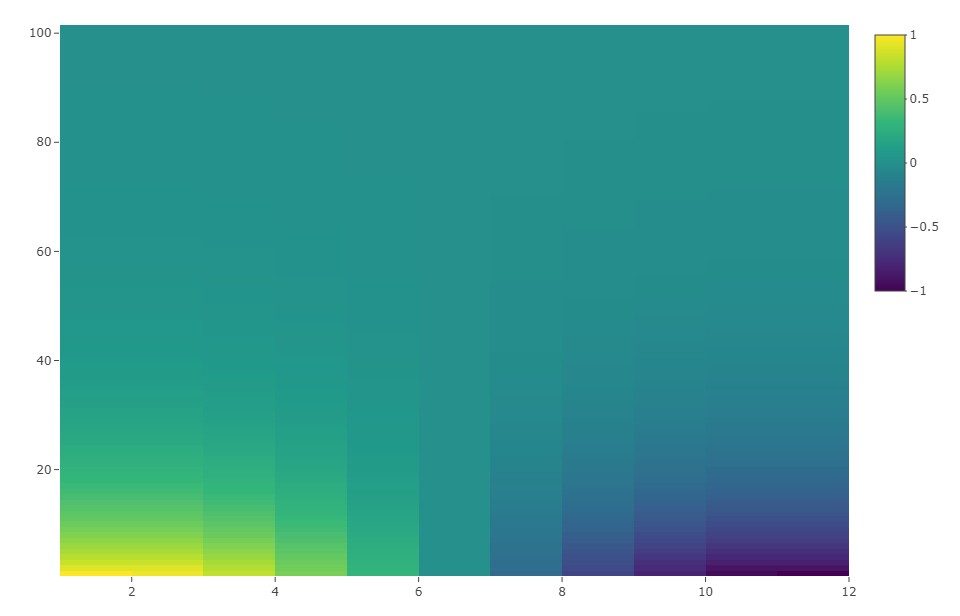
\includegraphics[width=6.5cm]{dyfuzjan.png}
    \caption{Dyfuzja na odcinku dla zagadnienia (8) z wykorzystaniem automatu komórkowego}
    \label{fig:my_label}
\end{figure}
\newpage
\subsubsection{Zagadnienie z mieszanymi warunkami brzegowymi}
Rozważamy układ równań różniczkowych z mieszanymi warunkami brzegowymi:
\begin{equation}
  \begin{array}{llll}
    u_t(z,t)&=&u_{xx}(x,t),&x\in(0,1),\\
    u(x,0)&=&\sin\pi x,\\
    u(0,t)&=&0,&u(1,t)=1.
    \end{array}
\end{equation}
To zagadnienie ma bardzo podobne warunki brzegowe jak zagadnienie (7), dlatego automat komórkowy z nim związany działa analogicznie. Wiadomo, że zagadnienie (9) ma rozwiązanie, które można znaleźć przy pomocy szeregów Fouriera \cite{str}.
\begin{tw}
Rozwiązanie zagadnienia (9) zbiega do rozwiązania zagadnienia stacjonarnego
\begin{equation}
    \begin{array}{cccc}
    \ w_{xx}&=&0,& x\in(0,1)\\
    w(0,t)&=&0,\\
    w(1,t)&=&1,
    \end{array}
\end{equation}
które dane jest wzorem
$$w(x)=x.$$
\end{tw}
\textbf{Dowód}\\
Poniższy dowód dla Twierdzenia 2 powstał z pomocą książki \cite{str}.
Niech $u(x,t)$ będzie rozwiązaniem zagadnienia (9), natomiast $w(x,t)$ rozwiązaniem dla (10). Wtedy $z(x,t)=u(x,t)-w(x,t)$ spełnia zagadnienie:
\begin{equation}
    \begin{array}{cccc}
    z_t(x,t)&=&z_{xx}(x,t),& x\in(0,1)\\
    z(x,0)&=&\sin\pi x - x,\\
    z(0,t)&=&0, &z(1,t)=0,\\
       \end{array}
\end{equation}
Przy mnożeniu $z_t-z_{xx}=0$ przez $z$ dostajemy
$$0=0z=(z_t-z_{xx})(z)=\frac{1}{2}(z^2)_t-(z_xz)_x+(z_x)^2.$$
Po nałożeniu całki na całe wyrażenie otrzymujemy
$$0 = \frac{1}{2}\int_0^1(z^2(x,t))_tdx -  z_x(1,t)z(1,t) + z_x(0,t)z(0,t) +\int_0^1(z_x(x,t))^2dx,$$
gdzie $z_x(1,t)z(1,t) - z_x(0,t)z(0,t)=0$ z warunków brzegowych. Zatem otrzymujemy
$$\frac{d}{dt}\int_0^1z^2(x,t)dx=-2\int_0^1(z_x(x,t))^2dx.$$
Dalej korzystając z nierówności Poincar\'ego 
$$\int^1_0z^2(x,t)dx\leq c\int_0^1\Big(z_x(x,t)\Big)^2dx,$$
dla prawej strony równania (zob. \cite{ev}, Ch. 5.6, Thm 3)  
$$\frac{d}{dt}\int_0^1z^2(x,t)dx=-2\int_0^1(z_x(x,t))^2dx\leq-2c\int_0^1(z(x,t))^2dx,$$
gdzie $c$ jest stała. Z tej nierówności różniczkowej wynika, że
$$\int_0^1z^2(x,t)dx\leq e^{-2ct}\int_0^1z^2(x,0)dx.$$
Wynika stąd, że $$\frac{d}{dt}\int_0^1z^2(x,t)dx\rightarrow0, \textrm{ gdy } t\rightarrow\infty\textrm{ wykładniczo.}$$
\#\\\\
Przyjmijmy, jak w poprzednich przykładach, że odcinek jest nagrzanym prętem. Dla zagadnienia (9) jeden koniec jest cały czas zimny, a drugi gorący. W związku z tym temperatura będzie się jednostajnie rozchodzić od jednego końca do drugiego. Na rysunku 18 bardzo dobrze widać, że w raz z upływem czasu rozwiązanie zbiega do funkcji liniowej.
\begin{figure}[!htb]
    \centering
    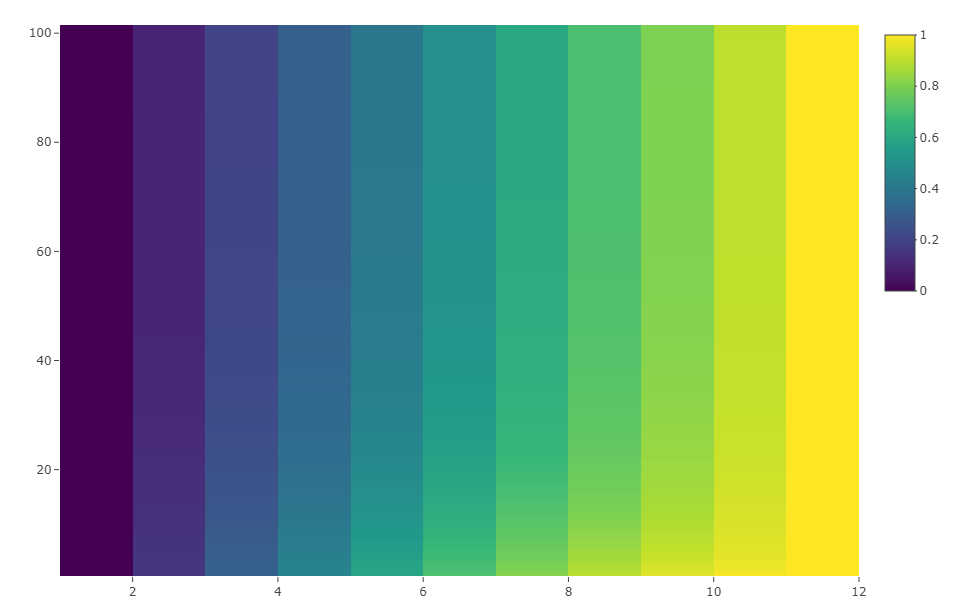
\includegraphics[width=6.5cm]{dyfuzja.png}
    \caption{Dyfuzja na odcinku dla zagadnienia (9) z wykorzystaniem automatu komórkowego}
    \label{fig:my_label}
\end{figure}
\newpage
\subsection{Kod do symulacji w R dla dyfuzji na odcinku z warunkami brzegowymi Dirichleta (rys. 35, 37) }
\begin{verbatim}
#Deklaracje zmiennych i ustalenie warunków początkowych:
 
dt <- 0.01
dx <- 0.1  
t <- 1
rows <- length(seq(0,t,dt))
columns <- length(seq(0,1,dx))
pi_value <- 3.14
M <- matrix(nrow=rows,ncol=columns)

#warunek początkowy
M[1,] <- sin(pi_value*seq(0,1,dx))

#warunki brzegowe Dirichleta (lub mieszane)
M[,1] <- 0
M[,columns] <- 0 # rys.35
M[,columns] <- 1 # rys.37

#Liczenie:

  for(i in seq(2,rows,1)){
    for(j in seq(2, columns-1, 1)){
      M[i,j] <- (M[i-1, j+1] + M[i-1, j-1])/2
        }
  }
  
#symulacje
plot_ly(
  x = c(1:100), y = c(1:100),
  z = M,  type = "heatmap" )
\end{verbatim}


\subsection{Kod do symulacji w R dla dyfuzji na odcinku z warunkami brzegowymi Neumanna (rys. 36)}

\begin{verbatim}
#Deklaracje zmiennych i ustalenie warunków początkowych:

dt <- 0.01
dx <- 0.1  
t <- 1
rows <- length(seq(0,t,dt))
columns <- length(seq(0,1,dx))
pi_value <- 3.14
M <- matrix(nrow=rows,ncol=columns)

#warunek początkowy
M[1,] <- cos(pi_value*seq(0,1,dx))

#Liczenie:

for(i in seq(2,rows,1)){
  for(j in seq(2, columns-1, 1)){
    M[i,j] <- (M[i-1, j+1] + M[i-1, j-1])/2
  }
#Warunki brzegowe Neumanna - brak przepływu przez brzeg
  M[i,1] <- M[i,2]
  M[i, columns] <- M[i, columns - 1]
}

#symulacje
plot_ly(
  x = c(1:100), y = c(1:100),
  z = M,  type = "heatmap" )


\end{verbatim}
\newpage
\section{Równania reakcji-dyfuzji}
\subsection{Opis teoretyczny modelu}
Układ Brusselator jest przykładem modelu dla reakcji-dyfuzji, opisującym autokatalizę dwóch związków chemicznych. 
Niech $u$ i $v$ symbolizują stężenie obydwu substancji. Załóżmy, że $u=u(x,t)$, $v=v(x,t)$ oraz $x\in[0,1].$ Brusselator to układ równań różniczkowych:
\begin{equation}
\begin{array}{lll}
u_t = D_uu_{xx}+A-(B+1)u+u^2v,&x\in(0,1),&t>0 &
v_t = D_vv_{xx}+Bu-u^2v,& x\in(0,1),& t>0 &
\end{array} 
\end{equation}
rozważany z warunkami początkowymi
$$u(x,0)=u_0(x)\geq0\textrm{ i } v(x,0)=v_0(x)\geq0,$$
a także warunkami brzegowymi Neumanna
$$u_x(0,t)=u_x(1,t)=0,\ v_x(0,t)=v_x(1,t)=0,$$
które zapewniają brak przepływu przez brzeg. Wyrażenia $D_u$, $D_v$ to stałe dyfuzji odpowiednio dla funkcji $u$ i $v$.\\ 
W związku z tym, że stanami stacjonarnymi naszego układu równań różniczkowych są $u=A$ i $v=\frac{B}{A}$, to symulacje będziemy przeprowadzać dla warunków początkowych, które są małym zaburzeniem tego rozwiązania stacjonarnego.

\subsection{Automat komórkowy dla układu Brusselator}
Aby zdefiniować☺ automat komórkowy dla równań reakcji dyfuzji, konieczne będzie wprowadzenie dodatkowej funkcji przejścia, a także rozróżnienia stanów w zależności od obiektu, który będziemy chcieli wykorzystać. W układzie Brusselator potrzebujemy opisać zmiany jakie zachodzą dla dwóch różnych związków chemicznych, z tego powodu automat komórkowy dla tego układu będzie postaci $A=(G, E, U, f, g)$. Przyjmijmy, że:
\begin{itemize}
    \item $G=\mathbb{Z}$ - jednowymiarowa siatka,
    \item $E=\mathbb{R}$ - zbiór stanów,
    \item $U(x_i)= \{x_{i-1}, x_i,x_{x+1}\}$ - sąsiedztwo komórki $x_i$,
    \item $\tau_1,\tau_2$ - stany komórek odpowiednio dla pierwszego i drugiego związku chemicznego,
    \item $f(\tau_1(\cdot,t)|_{U(x)})= D_u\frac{\tau_1(x_{i + 1}, t_k)+\tau_1(x_{i-1},t_k) }{2} + A - (B+1)\tau_1(x_i,t_k) + \tau_1^2(x_i,t_k)\tau_2(x_i,t_k)$ - funkcja przejścia dla pierwszego związku chemicznego,
    \item $g(\tau_2(\cdot,t)|_{U(x)})= D_v\frac{\tau_2(x_{i + 1}, t_k)+\tau_2(x_{i-1},t_k) }{2} + B\tau_1(x_i,t_k) - \tau_1^2(x_i,t_k)\tau_2(x_i,t_k)$ - funkcja przejścia dla drugiego związku chemicznego,
\end{itemize}
natomiast $D_u$ i $D_v$ są współczynnikami dyfuzji, $A,\ B$ są stałe.\\
Odcinek $[0,1]$ został podzielony na 100 komórek. Warunki początkowe dla pierwszego związku chemicznego zostały ustawione dla wszystkich komórek, z wyłączeniem komórek $x_{15}-x_{20},\ x_{45}-x_{60},\ x_{75}-x_{90}$, które przyjmują wartość $A+0.1$, na wartość równą $A$. Dla drugiego związku chemicznego warunek początkowy ustawiany jest na stałym poziomie równym $\frac{B}{A}$.
\subsection{Symulacje}
Zaprezentowane symulacje przedstawiają ewolucje układu (10), w zależności od dobranych parametrów, które są podane przy każdym rysunku. W kodzie do symulacji zostały wprowadzone dwie dodatkowe zmienne, które odpowiadają za:
\begin{itemize}
    \item $dt$ - krok czasu,
    \item $dx$ - wielkość komórek.
\end{itemize}
Dla poniższych symulacji mamy $$dt=0.1,\textrm{ a }dx=0.01.$$
\begin{figure}[hb]
\centering
\subfloat[$u(x,t)$]{\label{odnosnik}
\includegraphics[width=0.4\textwidth]{U_małeDU_A=B.png}}
\quad
\subfloat[$v(x,t)$]{\label{odnosnik}
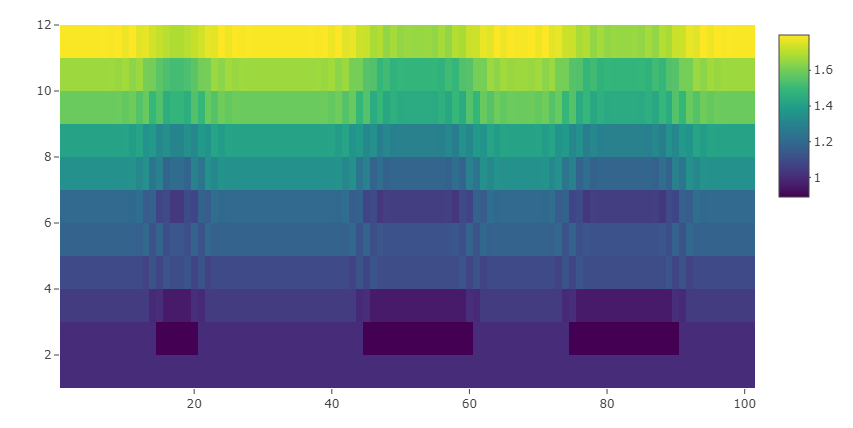
\includegraphics[width=0.4\textwidth]{V_maleDU_A=B.png}}
\caption{Ewolucja układu (10) z wykorzystaniem automatu komórkowego, z parametrami $A=B=1,\ D_u=0.05,\ D_v=1$. Możemy zaobserwować niejednorodne struktury pojawiające się w kolejnych iteracjach.}
\label{fig:animals}
\end{figure}
\newpage
\begin{figure}[bh]
\centering
\subfloat[$u(x,t)$]{\label{odnosnik}
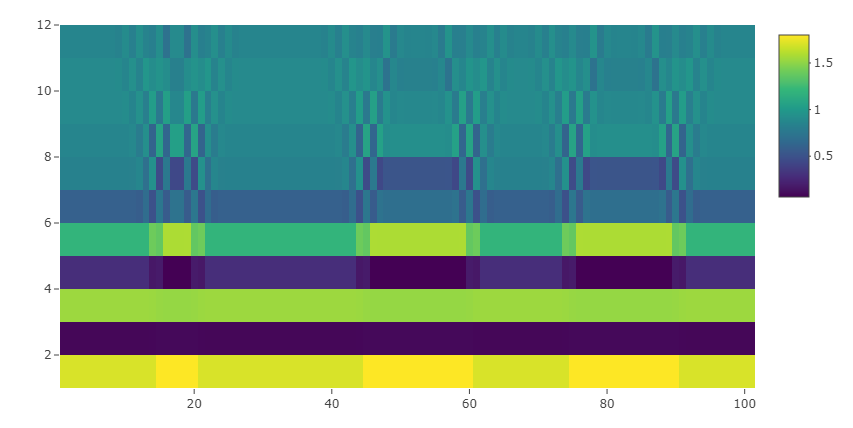
\includegraphics[width=0.4\textwidth]{U_maleDU_duzeA.png}}
\quad
\subfloat[$v(x,t)$]{\label{odnosnik}
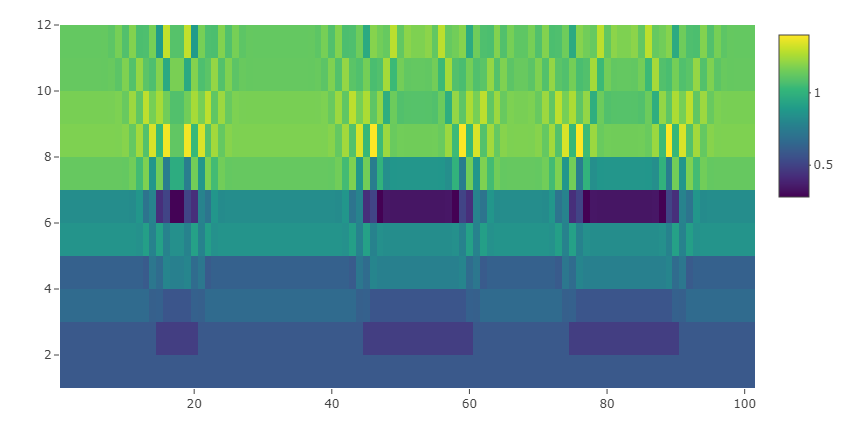
\includegraphics[width=0.4\textwidth]{V_maleDU_duzeA.png}}
\caption{Ewolucja układu (10) z wykorzystaniem automatu komórkowego, z parametrami $A=1.7,\ B=1,\ D_u=0.05,\ D_v=1$.}
\label{fig:animals}
\end{figure}

\begin{figure}[h]
\centering
\subfloat[$u(x,t)$]{\label{odnosnik}
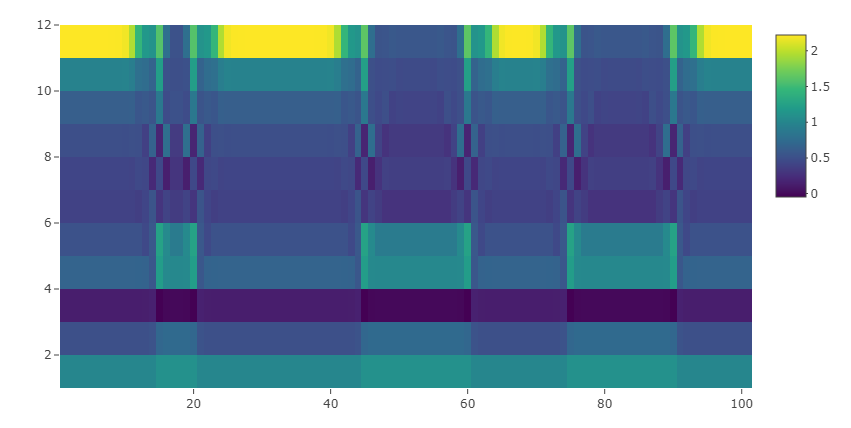
\includegraphics[width=0.4\textwidth]{U_duzeB.png}}
\quad
\subfloat[$v(x,t)$]{\label{odnosnik}
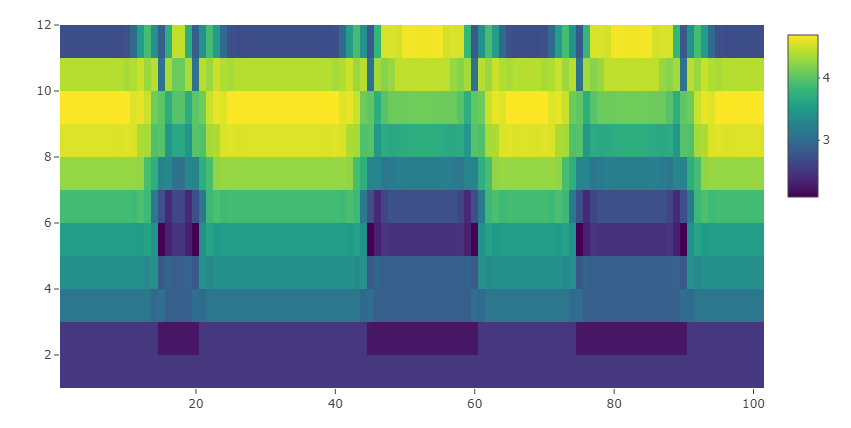
\includegraphics[width=0.4\textwidth]{V_duzeB.png}}
\caption{Ewolucja układu (10) z wykorzystaniem automatu komórkowego, z parametrami $A=1,\ B=2.5,\ D_u=0.5,\ D_v=1$. Przedstawiono tu niestabilność układu. Widzimy, że wraz z upływem czasu wartości zaczynają zbiegać, w niekontrolowany sposób do nieskończoności. Powodem takiego zachowania układu jest zbyt duża wartość parametru $B$, w porównaniu z $A$.}
\label{fig:animals}
\end{figure}

\newpage
\subsection{Kod do symulacji dla reakcji dyfuzji}

\begin{verbatim}    
#Deklaracje zmiennych i ustalenie warunków początkowych 
(zmieniane w zależności od rysunków, tu dla rysunku 40):

A <- 1 
B <- 2.5 
Du <- 0.5
Dv <-  1 
dt <- 0.1
dx <- 0.01  

rows <- length(seq(0,1,dt))
columns <- length(seq(0,1,dx))

U <- matrix(nrow=rows,ncol=columns)
V <- matrix(nrow=rows,ncol=columns)

#Warunki początkowe:

U[1,] <- A 
U[1,c(15:20, 45:60, 75:90)] <- A + 0.1
V[1,] <- B/A

#Liczenie:

for(i in seq(2,rows,1)){
  for(j in seq(2, columns-1, 1)){
  
    U[i,j] <- Du*(U[i-1, j+1] + U[i-1, j-1])/2 +
    + (A - (B+1)*U[i-1,j] + (U[i-1,j]*U[i-1,j])*V[i-1,j])
    
    V[i,j] <- Dv*(V[i-1, j+1] + V[i-1, j-1])/2 + (B*U[i-1,j] + 
    - (U[i-1,j]*U[i-1,j])*V[i-1,j])
  }
  #Warunki brzegowe Neumanna - brak przepływu przez brzeg:
  U[i,1] <- U[i,2]
  U[i, columns] <- U[i, columns - 1]
  V[i,1] <- V[i,2]
  V[i, columns] <- V[i, columns - 1]
}

#Symulacje:
plot_ly(
  x = c(1:100), y = c(1:100),
  z = U,  type = "heatmap" )
plot_ly(
  x = c(1:100), y = c(1:100),
  z = V,  type = "heatmap" )
\end{verbatim}

\section{Dodatek}
W tym rozdziale prezentuje, kody napisane w \verb R, przy pomocy \verb {RStudio}.  Wyniki ich działania zostały przedstawione na rysunkach zamieszczonych w pracy licencjackiej.

\subsection{Symulacje w 1D}
\subsubsection{Zasada 254}
\begin{verbatim}

M1 = matrix( nrow = 29, ncol = 49 )
M1[ , ] = 0
M1[1, 25] = 1

for ( i in 2:29 ){
  
  for ( j in 2:48 ){
    
    if ( M1[i-1, j-1] + M1[i-1, j] + M1[i-1, j+1] >= 1 )
    
    M1[i, j] = 1 
    
    else
    
    M1[i, j] = 0 
    
  }
  
#warunki brzegowe
  
  if ( M1[i-1, 2] == 1 )
  
    M1[i, 1] = 1
    
  else 
  
    M1[i, 1] = 0 
  
  if ( M1[i-1, 48] == 1 )
  
    M1[i, 49] = 1
    
  else
  
    M1[i, 49] = 0 

}

rule254 <- plot_ly(
        x = c(1:49), y = c(1:49),
        z = M1, type = "heatmap" )

\end{verbatim}
\subsubsection{Zasada 50}
\begin{verbatim}

M2 = matrix( nrow=29, ncol=49 )
M2[ , ] = 0
M2[1, 25] = 1

for (i in 2:29){
  
  for (j in 2:48){
    
    if ( (M2[i-1, j-1] + M2[i-1, j] + M2[i-1, j+1] >= 1) & (M2[i-1, j] == 0) )
    
      M2[i, j]= 1
      
    else
    
      M2[i, j]=0
  }
  #warunki brzegowe
  
  if ( (M2[i-1, 2] == 1) & (M2[i-1, 1] == 0) )
  
    M2[i, 1] = 1
    
  else 
  
    M2[i, 1] = 0
  
  if ( (M2[i-1, 48] == 1) & (M2[i-1, 49] == 0) )
  
    M2[i, 49] = 1
    
  else
  
    M2[i, 49] = 0
  
}


rule50 <- plot_ly(
  x = c(1:49), y = c(1:49),
  z = M2, type = "heatmap" )
\end{verbatim}
\subsubsection{Zasada 90}
\begin{verbatim}

M3 = matrix( nrow=29, ncol=49 )
M3[ , ] = 0
M3[1, 25] = 1

for ( i in 2:29 ){
  
 for ( j in 2:48 ){
 
  if ( (( M3[i-1, j-1] + M3[i-1, j] + M3[i-1, j+1] == 1 ) 
   & ( M3[i-1, j] == 0 )) || (( M3[i-1, j-1] + M3[i-1, j] + M3[i-1, j+1] == 2 )
   & ( M3[i-1, j] == 1 )) )
    
      M3[i, j] = 1
      
    else
    
      M3[i, j] = 0
    
  }
  #warunki brzegowe
  
  if ( M3[i-1, 2] == 1 )
    M3[i, 1] = 1
  else 
  
    M3[i, 1] = 0
  
  if ( M3[i-1, 48] == 1 )
  
    M3[i, 49] = 1
    
  else
  
    M3[i, 49] = 0
  
}

rule90 <- plot_ly(
  x = c(1:49), y = c(1:49),
  z = M3, type = "heatmap" )
  
\end{verbatim}

\subsection{Symulacje w 2D}
\subsubsection{Mrówka Langton'a}
\begin{verbatim}

ti = 15000
x_ax = length( seq(0,49,1) )
y_ax = length( seq(0,49,1) )

time = length( seq(0,ti,1) )

Mr = array(NA, dim = c(x_ax, y_ax, time) )
Mr[ , , ] = 0

#zadać warunek początkowy

Mr[25, 25, 1] = 2
Mr[25, 24, 2] = 2
Mr[25, 25, 2] = 1

#przechodzenie do nowej komórki i zamiana kolorów

for( t in seq(2, time-1 , 1) ){
  
  for( x in seq(2, x_ax-1, 1) ){
    
    for( y in seq(2, y_ax-1, 1) ){
      
      if ( (Mr[y, x, t] == 1) & (Mr[y, x-1, t] != 2) & (Mr[y, x+1, t] != 2)
         & (Mr[y-1, x, t] != 2) & (Mr[y+1, x, t] != 2) ){
         
       Mr[y, x, t+1] = 1 }
      
      if ( (Mr[y, x, t] == 0) & (Mr[y, x-1, t] != 2) & (Mr[y, x+1, t] != 2)
         & (Mr[y-1, x, t] != 2) & (Mr[y+1, x, t] != 2) ){
         
       Mr[y, x, t+1] = 0 }
    
      #1. Mrówka przyszła z lewej strony na komórkę w stanie 0,
          przechodzi do góry, komórka zmienia stan na 1.
      
      if( (Mr[y, x, t] == 2 ) & (Mr[y, x-1, t-1] == 2)
        & (Mr[y, x, t-1] == 0) ){ 
        
         Mr[y+1, x, t+1] = 2
         Mr[y, x, t+1] = 1 
         Mr[y-1, x, t+1] = Mr[y-1, x, t] 
         Mr[y, x+1, t+1] = Mr[y, x+1, t] 
         Mr[y, x-1, t+1] = Mr[y, x-1, t] }
        
      #2. Mrówka przyszła z lewej strony na komórkę w stanie 1,
          przechodzi w dol, komórka zmienia stan na 0.
      
      if( (Mr[y, x, t] == 2) & (Mr[y, x-1, t-1] == 2)
        & (Mr[y, x, t-1] == 1) ){
      
         Mr[y-1, x, t+1] = 2
         Mr[y, x, t+1] = 0
         Mr[y+1, x, t+1] = Mr[y+1, x, t] 
         Mr[y, x+1, t+1] = Mr[y, x+1, t] 
         Mr[y, x-1, t+1] = Mr[y, x-1, t] }
        
      #3. Mrówka przyszła z prawej strony na komórkę w stanie 0,
          przechodzi w dol, komórka zmienia stan na 1.
        
      if( (Mr[y, x, t] == 2) & (Mr[y, x+1, t- 1] == 2)
        & (Mr[y, x, t-1] == 0) ){
        
          Mr[y-1, x, t+1] = 2
          Mr[y, x, t+1] = 1 
          Mr[y+1, x, t+1] = Mr[y+1, x, t] 
          Mr[y, x+1, t+1] = Mr[y, x+1, t] 
          Mr[y, x-1, t+1] = Mr[y, x-1, t] }
          
      #4. Mrówka przyszła z prawej strony na komórkę w stanie 1,
          przechodzi do góry, komórka zmienia stan na 0.
      
      if( (Mr[y, x, t] == 2) & (Mr[y, x+1, t-1] == 2)
        & (Mr[y, x, t-1] == 1) ){
        
          Mr[y+1, x, t+1] = 2
          Mr[y, x, t+1] = 0
          Mr[y-1, x, t+1] = Mr[y-1, x, t] 
          Mr[y, x+1, t+1] = Mr[y, x+1, t] 
          Mr[y, x-1, t+1] = Mr[y, x-1, t] }    
          
      #5. Mrówka przyszła z dołu na komórkę w stanie 0, przechodzi w lewo,
          komórka zmienia stan na 1.
      
      if( (Mr[y, x, t] == 2) & (Mr[y-1, x, t-1] == 2) 
        & (Mr[y, x, t-1] == 0) ){
        
          Mr[y, x-1, t+1] = 2
          Mr[y, x, t+1] = 1 
          Mr[y-1, x, t+1] = Mr[y-1, x, t] 
          Mr[y, x+1, t+1] = Mr[y, x+1, t] 
          Mr[y+1, x, t+1] = Mr[y+1, x, t] }
          
      #6. Mrówka przyszła z dołu na komórkę w stanie 1, przechodzi w prawo, 
          komórka zmienia stan na 0.
      
      if( (Mr[y, x, t] == 2) & (Mr[y-1, x, t-1] == 2) 
        & (Mr[y, x, t-1] == 1 ) ){
        
          Mr[y, x+1, t+1] = 2
          Mr[y, x, t+1] = 0 
          Mr[y-1, x, t+1] = Mr[y-1, x, t] 
          Mr[y+1, x, t+1] = Mr[y+1, x, t] 
          Mr[y, x-1, t+1] = Mr[y, x-1, t] } 
          
      #7. Mrówka przyszła z góry na komórkę w stanie 0, przechodzi w prawo,
          komórka zmienia stan na 1.
      
      if( (Mr[y, x, t] == 2) & (Mr[y+1, x, t-1] == 2)
        & (Mr[y, x, t-1] == 0) ){
        
          Mr[y, x+1, t+1] = 2
          Mr[y, x, t+1] = 1 
          Mr[y-1, x, t+1] = Mr[y-1, x, t] 
          Mr[y+1, x, t+1] = Mr[y+1, x, t] 
          Mr[y, x-1, t+1] = Mr[y, x-1, t] }         
            
      #8. Mrówka przyszła z góry na komórkę w stanie 1, przechodzi do góry,
          komórka zmienia stan na 0.
      
      if( (Mr[y, x, t] == 2) & (Mr[y+1, x, t-1] == 2) 
        & (Mr[y, x, t-1] == 1) ){
        
          Mr[y, x-1, t+1] = 2
          Mr[y, x, t+1] = 0
          Mr[y-1, x, t+1] = Mr[y-1, x, t] 
          Mr[y, x+1, t+1] = Mr[y, x+1, t] 
          Mr[y+1, x, t+1] = Mr[y+1, x, t] }
      
    }
  }
}
plot_ly(
  x = c(1:49), y = c(1:49),
  z = Mr[,,t], colors = colorRamp(c("khaki", "darkgreen")), type = "heatmap" )

\end{verbatim}
t - krok, który chcemy wygenerować.
\subsubsection{Gra w życie}
\begin{verbatim}

ti = 2000
xc = length( seq(0, 75, 1) )
yc = length( seq(0, 75, 1) )

time = length( seq(0, ti, 1) )

G = array(NA, dim = c(xc, yc, time))
G[, , ] = 0

#zadać warunek początkowy 

#losowe wartości tablicy


v = c(1:100)

for(y in seq(1, 100 , 1)){
  
  G[ y, sample( v, sample(v[15:45], 1) ), 1 ] = 1
}

#pojedyncze wzory 

#pasy 75x75

G[35, c(15:54),1] = 1
G[35, c(24, 30:32, 36:42, 59), 1] = 0

#pulsar 25x25
 
G[c(7, 12, 14, 19), c(9:11, 15:17), 1] = 1
G[c(9:11, 15:17), c(7, 12, 14, 19), 1] = 1

#statki + stałe wzory

G[8, c(20:23), 1] = 1
G[9, c(19:23), 1] = 1
G[9, 21, 1] = 0
G[10, c(20, 21), 1] = 1
G[7, c(21, 22), 1] = 1

G[c(18, 19), 19, 1] = 1
G[20, c(18, 20), 1] = 1
G[19, 18, 1] = 1

G[c(18, 19), 4, 1] = 1
G[c(20, 19), 5, 1] = 1
G[20, 3, 1] = 1

#przechodzenie do nowej komórki i zamiana kolorów

for( t in seq(1, time-1 , 1) ){
  
  sr1 = G[1,2,t] + G[2, 2, t] + G[2, 1, t] + G[1, 1, t]
  sr2 = G[1, xc-1,t] + G[2, xc-1 , t] + G[2, xc, t] + G[1, xc, t]
  sr3 = G[yc, 1,t] + G[yc-1, 2, t] + G[yc-1, 1, t] + G[yc, 1, t]
  sr4 = G[yc, xc-1,t] + G[yc-1, xc, t] + G[yc-1, xc-1, t] + G[yc, xc, t]
  
  if(sr1 == 1) G[1, 1, t+1] = 1 else G[1, 1, t+1] = 0
  if(sr2 == 1) G[1, xc, t+1] = 1 else G[1, xc, t+1] = 0
  if(sr3 == 1) G[yc, 1, t+1] = 1 else G[yc, 1, t+1] = 0
  if(sr4 == 1) G[yc, xc, t+1] = 1 else G[yc, xc, t+1] = 0
  
  for( x in seq(2, xc-1, 1) ){
    
    S1 = G[1, x+1, t] + G[1, x-1, t] + G[2, x, t] + G[2, x-1, t] + G[2, x+1, t] + G[1, x, t]
    S2 = G[x+1, 1, t] + G[x-1, 1, t] + G[x, 2, t] + G[x-1, 2, t] + G[x+1, 2, t] + G[x, 1, t]
    S3 = G[yc, x+1, t] + G[yc, x-1, t] + G[yc-1, x, t] + G[yc-1, x-1, t]
       + G[yc-1, x+1, t] + G[yc, x, t]
    S4 = G[x+1, xc, t] + G[x-1, xc, t] + G[x, xc-1, t] + G[x-1, xc-1, t] 
       + G[x+1, xc-1, t] + G[x, xc, t]
    
    if(S1 == 2)  G[1, x, t+1] = 1 else  G[1, x, t+1] = 0
    if(S2 == 2)  G[x, 1, t+1] = 1 else  G[x, 1, t+1] = 0
    if(S3 == 2)  G[yc, x, t+1] = 1 else  G[1, x, t+1] = 0
    if(S4 == 2)  G[x, xc, t+1] = 1 else  G[x, xc, t+1] = 0
    
    for( y in seq(2, yc-1, 1) ){
      
      S = G[y-1, x, t] + G[y+1, x, t] + G[y, x-1, t] + G[y, x+1, t] 
      + G[y-1, x-1 ,t] + G[y-1, x+1, t] + G[y+1, x-1, t] + G[y+1, x+1, t] 

      if((S == 3)||((S == 2) & (G[y, x, t] == 1))) G[y, x, t+1] = 1 
      else   G[y, x, t+1] = 0
    }
  }
}

plot_ly(
  x = c(1:100), y = c(1:100),
  z = G[, ,t], colors = colorRamp(c("khaki", "darkgreen")), type = "heatmap" )
 
\end{verbatim}
t - krok, który chcemy wygenerować.

\section{Bibliografia}
\begin{thebibliography}{99}
\bibitem{hill} G. de Vries, T. Hillen, M. Lewis, B. Schõnfisch, J. M\"uller, A Course in Mathematical Biology: Quantitative Modeling with Mathematical and Computational Methods, Society for Industrial and Applied Mathematics, 2006;
\bibitem{mr} http://www2.udec.cl/~angajardo/langton/general.html;
\bibitem{loop} http://pti.krakow.pl/wp-content/uploads/prezentacjaPTI.pdf;
\bibitem{l} Weisstein, Eric W. „Mrówka Langtona”. Z MathWorld - zasób sieciowy Wolfram. https://mathworld.wolfram.com/LangtonsAnt.html;
\bibitem{200} A. Gajardo, A. Moreira, E. Goles, "Complexity of Langton's ant" (PDF). Discrete Applied Mathematics. 2002;
\bibitem{2015} https://www.conwaylife.com/ref/lexicon/lex\_g.htm#gosperglidergun;
\bibitem{st} http://wwwhomes.uni-bielefeld.de/achim/moving.html;
\bibitem{o} http://entropymine.com/jason/life/status.html#oscper;
\bibitem{d} B. M. Jaworski, A. A. Dietłaf, Fizyka. Poradnik encyklopedyczny, Wydawnictwo Naukowe PWN, 2000;
\bibitem{g} M. Gardner, Mathematical Games, Scientific American, vol. 223, no. 4, 1970;
\bibitem{mb} J. D. Murray, Mathematical Biology, Springer-Verlag Nowy Jork, 2002;
\bibitem{rr} S. Olariu, A. Y. Zomaya, Handbook of Bioinspired Algorithms and Applications, Chapman and Hall/CRC, 2005;
\bibitem{gif} https://commons.wikimedia.org/wiki/File:Oscillator.gif;
\bibitem{lan}  C. G. Langton, Artificial life: an overview, MIT Press, 1998;
\bibitem{dyf} https://sjp.pwn.pl/sjp/dyfuzja;2555615.html;
\bibitem{str} W. A. Strauss, Partial differential equations: an introduction, John Wiley & Sons, Inc., 1992;
\bibitem{ev} L. C. Evans, Partial differential equations, American Mathematical Society, 1997;
\end{thebibliography}


\end{document}
